\documentclass[a4paper,fontsize = 7pt]{scrartcl}
\usepackage[utf8]{inputenc}
\usepackage[nswissgerman]{babel}

\usepackage{lipsum}

% Andrej Scheuer's Stuff
\usepackage{tikz}

\usetikzlibrary{positioning, calc, fit, matrix, decorations, angles, quotes, babel, 3d, arrows.meta, shadings, shapes.geometric}

\tikzset{>=stealth,
	overlaynote/.style={font = \footnotesize, fill = overlaycolor, draw = overlaycolor, rounded corners = 3pt},
	overlayarrow/.style={thick, gray, ->}
}


% 3 column landscape layout with fewer margins
\usepackage[landscape, left=0.75cm, top=1cm, right=0.75cm, bottom=1.5cm, footskip=5pt]{geometry}
\usepackage{flowfram}
\ffvadjustfalse
\setlength{\columnsep}{1cm}
\Ncolumn{4}

% define nice looking boxes
\usepackage[most]{tcolorbox}

% a base set, that is then customised
\tcbset {
  base/.style={
    boxrule=0mm,
    leftrule=1mm,
    left=1.75mm,
    arc=0mm, 
    fonttitle=\bfseries, 
    colbacktitle=black!10!white, 
    coltitle=black, 
    toptitle=0.75mm, 
    bottomtitle=0.25mm,
    title={#1}
  }
}

\definecolor{nicegreen}{rgb}{0.004, 0.5, 0.35}
\newtcolorbox{mainbox}[1]{
  colframe=nicegreen, 
  base={#1}
}

\newtcolorbox{subbox}[1]{
  colframe=black!20!white,
  base={#1}
}

% Mathematical typesetting & symbols
\usepackage{amsthm, mathtools, amssymb, centernot} 
\usepackage{marvosym, wasysym}
\allowdisplaybreaks

% Tables
\usepackage{tabularx, multirow}
\usepackage{booktabs}
\renewcommand*{\arraystretch}{2}

% Make enumerations more compact
\usepackage{enumitem}
\setitemize{itemsep=0.5pt}
\setenumerate{itemsep=0.75pt}

% To include sketches & PDFs
\usepackage{graphicx}


% For hyperlinks
\usepackage{hyperref}
\hypersetup{
  colorlinks=true
}

% Metadata
\title{Cheatsheet Analysis 1}
\author{Nicolas Wehrli}
\date{August 2022}

% Math helper stuff
\def\limn{\lim_{n\to \infty}}
\def\limxo{\lim_{x\to 0}}
\def\limxi{\lim_{x\to\infty}}
\def\limxn{\lim_{x\to-\infty}}
\def\sumk{\sum_{k=1}^\infty}
\def\sumn{\sum_{n=0}^\infty}
\def\Z{\mathbb{Z}}
\def\R{\mathbb{R}}
\def\N{\mathbb{N}}
\def\C{\mathbb{C}}
\def\dx{\text{ d}x}
\def\oof{\mathcal{O}}

%removing paragraph indent
\setlength{\parindent}{0cm}

\begin{document}

\maketitle

\section{Reelle Zahlen}
\subsection{Definiton und Axiome}
Die Menge $\R $ ist mit zwei Operatoren versehen: \\
Addition $+$: $\R \times \R \to \R:  (x,y) \to x+y$ 
\begin{subbox}{Axiome der Addition}
  \vspace{-6pt}
  A1 $\forall x,y,z \in \R: x+(y+z) = (x+y)+z$\\
  A2 $\exists 0\in\R: x + 0 = x, \forall x \in \R$\\
  A3 $\forall x \in \R, \exists y \in \R: x+y = 0$\\
  A4 $\forall x,y \in \R: x+y = y+x$
  \vspace{-6pt}
\end{subbox}
Multiplikation $\cdot$: $\R \times \R \to \R: (x,y) \to x\cdot y$

\begin{subbox}{Axiome der Multiplikation}
  \vspace{-6pt}
  A1 $\forall x,y,z \in \R: x\cdot(y \cdot z) = (x \cdot y)\cdot z$\\
  A2 $\exists 1\in\R: x \cdot 1 = x, \forall x \in \R$\\
  A3 $\forall x \in \R, \exists y \in \R: x \cdot y = 1$\\
  A4 $\forall x,y \in \R: x \cdot y = y \cdot x$
  \vspace{-6pt}
\end{subbox}

$\R$ ist ein angeordneter Körper.

\begin{subbox}{Ordnungsaxiome}
  \vspace{-6pt}
  O1 $\forall x \in \R: x \leq x$\\
  O2 $\forall x,y,z \in\R: x \leq y \land y \leq z \implies x \leq z$\\
  O3 $\forall x,y \in \R: x \leq y \land y \leq x \implies x = y$\\
  O4 $\forall x,y \in \R: x \leq y$ oder $y \leq x$\\
  Die Ordnung ist konsistent mit Addition und Multiplikation.\\
  K1: $\forall x,y,z \in \R : x \leq y \implies x + z \leq y + z$
  K2: $\forall x \in \R^{+}$ und $\forall y \geq 0$
  \vspace{-6pt}
\end{subbox}

\begin{mainbox}{Ordnungsvollständigkeit}
  \vspace{-4pt}
  Seien $A$ und $B$ Teilmengen von $\R$, so dass \\
  (i) $A \neq \emptyset, B \neq \emptyset$\\
  (ii) $\forall a \in A$ und $\forall b \in B$ gilt: $a \leq b$\\
  Dann gibt es (mindestens) ein $c \in \R$, so dass $\forall a \in A: a \leq c$ und $\forall b \in B: c \leq b$
  \vspace{-4pt}
\end{mainbox}

\begin{mainbox}{Archimedisches Prinzip}
  \vspace{-4pt}
  (1) Sei $x \in \R, x > 0$ und $y \in \R$. Dann gibt es $n \in \mathbb{N}$ mit $y \leq n \cdot x$ \\
  (2) Für jedes $x \in \R$ existiert genau ein $n \in \mathbb{Z}$ mit $n \leq x < n+1$
  \vspace{-4pt}
\end{mainbox}

\arraycolsep=0pt\def\arraystretch{1}
\begin{subbox}{Betragsrechenregeln}
  \vspace{-6pt}
  \begin{equation*}
      \begin{array}{rcl}
          (i) & |x| \geq 0 & \forall x \in \R\\
          (ii) & |xy| = |x||y| & \forall x,y \in \R\\
          (iii) & |x+y| \leq |x| + |y| & \forall x,y \in \R\\
          (iv) & |x+y| \geq ||x| - |y|| & \forall x,y \in \R
      \end{array}
  \end{equation*}
  \vspace{-10pt}
\end{subbox}

\begin{subbox}{Young'sche Ungleichung}
  \vspace{-4pt}
  $\forall \varepsilon>0, \forall x, y \in \R$ gilt $2 \cdot |x \cdot y| \leq \varepsilon \cdot x^2 + \frac{1}{\varepsilon} \cdot y^2$ 
  \\ \textit{Beweisidee:} $(\sqrt{\varepsilon}\cdot |x| - \frac{1}{\sqrt{\varepsilon}} \cdot |y|)^2 \geq 0$ 
  \vspace{-4pt}
\end{subbox}

Sei $A \subseteq \R, A \neq \emptyset$: 
\begin{itemize}
  \item $c \in \R$ ist eine \textbf{obere (untere) Schranke} von $A$ falls $\forall a \in A: a \leq (\geq) c$
  \item Ein Element $M \in \R$ ist ein \textbf{Maximum (Minimum)} von $A$ falls $M \in A, \forall a \in A: a \leq (\geq) M$
  \item Sei $A$ nach oben beschränkt. Die kleinste obere Schranke von $A$ ist das \textbf{Supremum} von $A$.
  \item Sei $A$ nach unten beschränkt. Die grösste untere Schranke von $A$ ist das \textbf{Infimum} von $A$.
  
  \item sup({$A \bigcup B$}) = max{(sup$A$, sup$B$)}
  \item sup{($A + B$)} = sup($A$) + sup($B$)
  \item sup($c \cdot A$) = $c \cdot $ sup($A$), $c > 0$
  \item sup($c \cdot A$) = $c \cdot$ Inf($A$), $c < 0$
\end{itemize}

\subsection{Euklidischer Raum}
\begin{equation*}
    \langle x, y \rangle = \sum_{i=1}^n x_i y_i \qquad ||x|| = \sqrt{\langle x,x \rangle}
\end{equation*}
\begin{subbox}{Cauchy-Schwarz}
  \vspace{-6pt}
    \begin{equation*}
        |\langle x, y \rangle| \leq ||x|| \cdot ||y|| \quad \forall x,y \in \R^n
    \end{equation*}
    \vspace{-16pt}
\end{subbox}
\begin{subbox}{1.22}
  \vspace{-4pt}
    \begin{enumerate}
        \item $||x|| \geq 0$ mit Gleichheit bei $x=0$.
        \item $||\alpha \cdot x|| = |\alpha|\cdot ||x|| \quad \forall \alpha \in \R,~\forall x \in \R^n$
        \item $||x+y|| \leq ||x|| + ||y|| \quad \forall x,y \in \R^n$
    \end{enumerate}
    \vspace{-12pt}
\end{subbox}

\subsection{Imaginäre Zahlen}
\begin{center}
  $i^2 = -1$\\
  $z := x + iy$ \qquad $\overline{z} := x - iy$\\
  $\text{Re}(z) := x \in \R$ \qquad  $\text{Im}(z) := y \in \R$
\end{center}
\begin{subbox}{1.24}
  \vspace{-4pt}
    \begin{enumerate}
        \item $\overline{(z_1 + z_2)} = \overline{z_1} + \overline{z_2}, \forall z_1,z_2 \in \R$  
        \item $\overline{(z_1 z_2)} = \overline{z_1} \overline{z_2},  \forall z_1,z_2 \in \mathbb{C}$
        \item $z\overline{z} = x^2 + y^2 = ||z||^2$
    \end{enumerate}
    \vspace{-12pt}
\end{subbox}
\begin{equation*}
    z^{-1} = \frac{\overline{z}}{||z||^2}
\end{equation*}
Polarform: $z = ( \cos \phi + i \sin \phi)$, wobei $r = ||z||$ der \emph{Absolutbetrag} und $\phi$ das \emph{Argument} von $z$.
\begin{mainbox}{Fundamentalsatz Algebra}
  \vspace{-4pt}
    $n \geq 1,~n\in \mathbb{N}$ und 
    \begin{equation*}
        P(z) = z^n + a_{n-1} z^{n-1} + \ldots + a_o \quad a_j \in \mathbb{C}
    \end{equation*}
    Dann gibt es $z_1, ..., z_n$ in $\mathbb{C}$, sodass
    \begin{equation*}
        P(z) = (z - z_1)(z - z_2) \ldots(z-z_n)
    \end{equation*}
    \vspace{-16pt}
\end{mainbox}
Eulersche Formel: $e^{i\phi} = \cos \phi + i \sin \phi$

\section{Folgen}
\subsection{Konvergenz}
Eine Folge $(a_n)_{n\in \mathbb{N}}$ konvergiert gegen L \\ $\iff \lim_{n \to \infty} a_n = L $ 
\\ $\iff \forall \varepsilon > 0 \ \exists N_\varepsilon \ \forall n \ge N_\varepsilon : \ | a_n - L | < \varepsilon$
\\ $\iff \forall \varepsilon > 0 $ ist die Menge ${n \in \N: a_n \notin ]l-\varepsilon,l+\varepsilon[}$ endlich. 
\\ Es gibt für eine konvergente Folge $(a_n)_{n \geq 1}$ höchstens ein $L \in \R$, dass diese Bedingungen erfüllt.


Wir dürfen (o.B.d.A.) annehmen, dass $\varepsilon $ durch eine Konstante $C \in \R$ beschränkt ist.
Es gilt ausserdem:
\begin{itemize}
 \item konvergent $\implies$ beschränkt, aber nicht umgekehrt
 \item $(a_n)$ konvergent $\iff (a_n)$ beschränkt \textbf{und} $\lim \inf a_n = \lim \sup a_n$
\end{itemize}

Sei $(a_n)_{n \geq 1}$, $(b_n)_{n \geq 1}$ konvergente Folgen. mit \\$\limn a_n = a, \limn b_n = b$ dann gilt:
\begin{itemize}
  \item $(a_n \pm b_n)_{n \geq 1}$ konvergent, $\limn (a_n \pm b_n) = a \pm b$
  \item $(a_n \cdot b_n)_{n \geq 1}$ konvergent, $\limn (a_n \cdot b_n) = a \cdot b$
  \item $(a_n \div  b_n)_{n \geq 1}$ konvergent, $\limn (a_n \div b_n) = a \div b$ ($b_n \neq 0, \forall n \in \N, b \neq 0$)
  \item Falls $\exists K \geq 1$ mit $a_n \leq b_n ~ \forall n \geq K$ folgt $a \leq b$
\end{itemize}

\begin{subbox}{Limes superior \& inferior}
  \vspace{-4pt}
$\limn \inf x_n = \limn \left( \inf_{m \ge n} x_m \right)$ \\
$\limn \sup x_n = \limn \left( \sup_{m \ge n} x_m \right)$
  \vspace{-12pt}
\end{subbox}

\begin{mainbox}{Einschliessungskriterium \\ (Sandwich-Theorem)}
  \vspace{-4pt}
Wenn $\limn a_n = \alpha, \ \limn b_n = \alpha$ und $a_n \le c_n \le b_n, \forall n \ge k$, dann $\limn c_n = \alpha$.
  \vspace{-4pt}
\end{mainbox}

\begin{mainbox}{Weierstrass}
Wenn $a_n$ monoton wachsend und nach oben beschränkt ist, dann konvergiert $a_n$ mit Grenzwert $\limn a_n = \sup \{a_n : \ n \ge 1\}$.

Wenn $a_n$ monoton fallend und nach unten beschränkt ist, dann konvergiert $a_n$ mit Grenzwert $\limn a_n = \inf \{a_n : \ n \ge 1\}$.
\end{mainbox}

\textbf{Tipp:} umschreiben $f(x)^{g(x)} = e^{g(x) \cdot \ln \left( f(x) \right)}$ und Grenzwert im Exponent berechnen (l'Hopital).
\begin{subbox}{	Berechne $\lim_{x \to 0^+} x^{\sin(x)}$.}
  \vspace{-6pt}
		$\lim_{x \to 0^+} x^{\sin(x)} = \lim_{x \to 0^+} e^{ \ln \left( x^{\sin(x)} \right)} 
    = \lim_{x \to 0^+} e^{\sin (x) \ln (x)}$
	\\$e^x$ ist stetig $\Rightarrow$ Limes in Exponent.
	$
		\lim_{x \to 0^+} \sin(x) \ln(x) = \lim_{x \to 0^+} \frac{\ln(x)}{\frac{1}{\sin(x)}}
		\\\overset{\text{H}}{=} \lim_{x \to 0^+} \frac{\frac{1}{x}}{\frac{-\cos (x)}{\sin^2 (x)}} = \lim_{x \to0^+} \frac{- \sin^2 (x)}{x \cos (x)}\\
						= \lim_{x \to 0^+} \frac{- \sin x}{x} \cdot \frac{\overset{\to 0}{\sin x}}{\underset{\to 1}{\cos x}} = 0
	$
	\\Daraus folgt: $\lim_{x \to 0^+} e^{\sin (x) \ln (x)} = e^0 = 1$
  \vspace{-4pt}
\end{subbox}

\begin{mainbox}{Bernoulli Ungleichung}
  \vspace{-4pt}
  $(1 + x)^n \geq 1 + n \cdot x \qquad \forall n \in \N, x > -1$
  \vspace{-4pt}
\end{mainbox}

\begin{mainbox}{Cauchy-Kriterium}
  \vspace{-4pt}
Die Folge $a_n$ ist genau dann konvergent, falls \\ $\forall \varepsilon > 0 \exists N \ge 1$ so dass $| a_n - a_m | < \varepsilon \quad \forall n,m \ge N$.
  \vspace{-4pt}
\end{mainbox}

\subsubsection{Teilfolge}
Eine Teilfolge von $a_n$ ist eine Folge $b_n$ wobei $b_n = a_{l(n)}$.
\\ $l$ ist eine Funktion mit $l(n) < l(n+1) \quad \forall n \ge 1$ (z.B. $l = 2n$ für jedes gerade Folgenglied). 

\begin{subbox}{Bolzano-Weierstrass}
Jede beschränkte Folge besitzt eine konvergente Teilfolge.
\end{subbox}
 \textbf{Wenn 2 Teilfolgen nicht den gleichen Grenzwert haben, impliziert das Divergenz.}

\subsection{Strategie - Konvergenz von Folgen}
\begin{enumerate}
 \item Bei Brüchen: Grösste Potenz von $n$ kürzen. Alle Brüche der Form $\frac{a}{n^a}$ streichen, da diese nach 0 gehen.
 \item Bei Wurzeln in Summe im Nenner: Multiplizieren des Nenners und Zählers mit der Differenz der Summe im Nenner. (z.B. $(a+b)$ mit $(a-b)$ multiplizieren)
 \item Bei rekursiven Folgen: Anwendung von Weierstrass zur monotonen Konvergenz
 \item Einschliessungskriterium (Sandwich-Theorem) anwenden.
 \item Mit bekannter Folge vergleichen.
 \item Grenzwert durch einfaches Umformen ermitteln.
 \item Limit per Definition der Konvergenz zeigen.
 \item Anwendung des Cauchy-Kriteriums.
 \item \textbf{Suchen eines konvergenten Majorant. ????}
 \item Weinen und die Aufgabe überspringen.
\end{enumerate}

\subsection{Strategie - Divergenz von Folgen}
\begin{enumerate}
 \item Suchen einer divergenten Vergleichsfolge.
 \item Alternierende Folgen: Zeige, dass Teilfolgen nicht gleich werden, also $\limn a_{p_1(n)} \ne \limn a_{p_2(n)}$ (mit z.B. gerade/ungerade als Teilfolgen).
\end{enumerate}

\subsection{Tricks für Grenzwerte}
\subsubsection{Binome}
$$\lim_{x\to\infty} (\sqrt{x + 4} - \sqrt{x - 2}) = \lim_{x\to\infty} \frac{(x+4)-(x-2)}{\sqrt{x+4}+\sqrt{x-2}}$$

\subsubsection{Substitution}
$$\lim_{x\to\infty} x^2 (1-\cos(\frac{1}{x}))$$
Substituiere nun $u = \frac{1}{x}$:
$$\lim_{u \to 0} \frac{1 - \cos(u)}{u^2} = \lim_{u \to 0} \frac{\sin(u)}{2u} = \lim_{u\to 0} \frac{\cos(u)}{2} = \frac{1}{2}$$

\subsubsection{Induktive Folgen (Induktionstrick)}
\begin{enumerate}
  \item Zeige monoton wachsend / fallend
  \item Zeige beschränkt
  \item Nutze Satz von Weierstrass, d.h. Folge muss gegen Grenzwert konvergieren
  \item Verwende Induktionstrick (um den Grenzwert zu finden):
\end{enumerate}
\textbf{Wenn die Folge konvergiert, hat jede Teilfolge den gleichen Grenzwert.} Betrachte die Teilfolge $l(n) = n + 1$ für $d_{n+1} = \sqrt{3d_n - 2}$:
$$d = \lim_{n\to\infty} d_n = \lim_{n\to\infty} d_{n+1} = \sqrt{\lim_{n \to \infty} 3d_n -2} = \sqrt{3d -2}$$
Forme um zu $ d^2 = 3d -2 \to d \in {1,2}$. Nun können wir $d = 2$ nehmen und die Beschränktheit mit $d=2$ per Induktion zeigen.

\section{Reihen}

\begin{mainbox}{Cauchy-Kriterium für Reihen}
  \vspace{-4pt}
Die Reihe $\sumk a_k$ ist genau dann konvergent, falls $\forall \varepsilon > 0 \ \exists N \ge 1$ mit $| \sum_{k=n}^m a_k | < \varepsilon, \ \forall m \ge n \ge N$.
  \vspace{-4pt}
\end{mainbox}

\begin{subbox}{Nullfolgenkriterium}
  \vspace{-4pt}
 Wenn für eine Folge $\limn |a_n| \ne 0$ ist, dann divergiert $\sumn a_n$.
 \vspace{-4pt}
\end{subbox}


\subsection{Reihenarithmetik}
Wenn $\sumk a_k$ und $\sumk b_k$ konvergent sind, dann gilt:
\begin{itemize}
 \item $\sumk (a_k + b_k)$ konvergent und $\sumk (a_k + b_k) = \left( \sumk a_k \right) + \left( \sumk b_k \right)$
 \item $\sumk \alpha a_k$ konvergent und \\$\sumk \alpha a_k = \alpha \sumk a_k$
\end{itemize}


\begin{mainbox}{Vergleichssatz}
  \vspace{-4pt}
Wenn $\sumk a_k$ und $\sumk b_k$ Reihen mit $0 \le a_k \le b_k, \forall k \ge K \ge 1$ sind, so gilt:
$$\sumk b_k \text{ konvergent} \implies \sumk a_k \text{ konvergent}$$ 
$$\sumk a_k \text{ divergent} \implies \sumk b_k \text{ divergent}$$ 
  \vspace{-12pt}
\end{mainbox}

Als Vergleichsreihe (Majorant / Minorant) eignet sich oft eine Reihe der folgenden Kategorien:
\subsubsection{Geometrische Reihe} 
$\sum_{k=0}^\infty q^k$ divergiert für $|q| \ge 1$ und konvergiert zu $\frac{1}{1 - q}$ für $|q| < 1$

(Beweis per Teleskopidee: $S_n - q \cdot S_n = (1-q) \cdot S_n = 1 - q^n$)
\subsubsection{Zeta-Funktion}
$\zeta(s) = \sum_{n=1}^\infty \frac{1}{n^s}$ divergiert für $s \le 1$ und konvergiert für $s > 1$.
\subsubsection{Teleskop Reihe}
Sei $S_n = \sum_{k=1}^{n} a_k - a_{k+1}$ eine Reihe. Dann gilt $S_n = a_1 - a_{n+1}$ und $\limn S_n = a_1 + \limn a_{n+1}$


\subsection{Absolute Konvergenz}
$\sumk a_k$ heisst \textbf{absolut konvergent}, wenn $\sumk |a_k|$ konvergiert. Es gilt $|\sumk a_k| \le \sumk |a_k|$.

Falls eine Reihe absolut konvergiert, dann konvergiert jede Umordnung der Reihe mit dem selben Grenzwert.

Falls die Reihe hingegen nur konvergiert, so gibt es immer eine Anordnung, so dass $\sum_{k=1}^\infty a_{\phi(k)} = x, \ \forall x\in \R, \phi: \N \to \N$ (Bijektion).

\begin{subbox}{Leibnizkriterium}
  \vspace{-4pt}
Wenn $a_n \ge 0, \ \forall n \ge 1$ monoton fallend ist und $\limn a_n = 0$ gilt, dann konvergiert $S = \sumk (-1)^{k+1} a_k$ und $a_1 - a_2 \le S \le a_1$.
(Geht auch für monton fallend $\forall n \geq N, N \in \N$, dann muss aber bei der Abschätzung alle Terme mit Index $k \leq N$ vorkommen)
  \vspace{-4pt}
\end{subbox}

\begin{mainbox}{Quotientenkriterium}
  \vspace{-4pt}
Sei $(a_n)$ eine Folge mit $a_n \ne 0, \forall n \ge 1$. \\ Falls $\limn \sup \frac{|a_{n+1}|}{|a_n|} < 1 \implies \sum_{n=1}^\infty a_n$ konvergiert absolut. \\Falls $\limn \inf \frac{|a_{n+1}|}{|a_n|} > 1 \implies \sum_{n=1}^\infty a_n$ divergiert.  
  \vspace{-4pt}
\end{mainbox}

\begin{mainbox}{Wurzelkriterium}
  \vspace{-4pt}
  Sei $(a_n)$ eine Folge mit $a_n \ne 0, \forall n \ge 1$. Sei $q = \limn \sup \sqrt[n]{|a_n|}$. 
\begin{itemize}
 \item $q < 1 \implies \sum_{n=1}^\infty a_n$ konvergiert absolut.
 \item $q = 1 \implies$ keine Aussage.
 \item $q > 1 \implies \sum_{n=1}^\infty a_n$ und $\sum_{n=1}^\infty |a_n|$ divergieren.
\end{itemize}
\vspace{-12pt}
\end{mainbox}

\subsection{Wichtige Reihen}
\begin{align*}
 \sum_{i=1}^n i &= \frac{n(n+1)}{2} \\
 \sum_{i=1}^n i^2 &= \frac{1}{6}n(n+1)(2n+1) \\
 \sum_{i=1}^n i^3 &= \frac{1}{4}n^2(n+1)^2 \\
 \sum_{i=1}^\infty \frac{1}{i^2} &= \frac{\pi^2}{6} \\
 \sum_{n=1}^\infty \frac{1}{n(n+1)} &= 1
\end{align*}

\subsection{Cauchy-Produkt}
\begin{subbox}{Definition Cauchy-Produkt}
  \vspace{-4pt}
  Das Cauchy-Produkt von zwei Reihen $\sum_{i = 0}^\infty a_i$ und $\sum_{j = 0}^\infty b_j$ ist definiert als
  $$\sum_{n=0}^\infty \sum_{j=0}^n (a_{n-j} \cdot b_j) = a_0b_0 + (a_0b_1 + a_1b_0) + \ldots$$ Es konvergiert, falls beide Reihen absolut konvergieren.
  \vspace{-4pt}
\end{subbox}

\subsection{Strategie - Konvergenz von Reihen}
\begin{enumerate}
 \item Ist Reihe ein bekannter Typ? (Teleskopieren, Geometrische/Harmonische Reihe, Zetafunktion, ...)
 \item Ist $\limn a_n = 0$? Wenn nein, divergent.
 \item Quotientenkriterium \& Wurzelkriterium anwenden
 \item Vergleichssatz anwenden, Vergleichsreihen suchen
 \item Leibnizkriterium anwenden
 \item Integral-Test anwenden (Reihe zu Integral)
\end{enumerate}

\subsection{Funktionenfolge}
Für jedes $n$, sei $f_n: \N \to \R$ eine Folge. $(f_n)_{n \geq 1}$ ist eine Folge der Folgen. 
Wir nehmen an, dass
\begin{enumerate}
  \item $f(j) := \limn f_n(j)$ existiert $\forall j \in \N$
  \item Es gibt eine Funktion $g: \N \to [0, \infty[$, so dass
  \begin{enumerate}
    \item $|f_n(j)| \leq g(j), \forall j \geq 0,\forall n \geq 0$
    \item $\sum_{j = 0}^{\infty} g(j)$ konvergiert.
  \end{enumerate}
\end{enumerate}

\begin{subbox}{}
  \vspace{-8pt}
  $$exp(z) = \sum_{n = 0}^{\infty} \frac{z^n}{n!} = \limn (1 + \frac{1}{n})^n$$
  \vspace{-12pt}
\end{subbox}

\section{Funktionen}
\subsection{Stetigkeit}
Sei $f : D \to \R^d, x \to f(x)$ eine Funktion in $D \subseteq \R^d$.
\begin{mainbox}{Definition Stetigkeit}
  \vspace{-4pt}
 $f$ ist in $x_0 \in D$ stetig, $\iff \forall \varepsilon > 0, \exists \delta > 0$, s.d. $|x-x_0|<\delta \to |f(x)-f(x_0)| < \varepsilon$
 \\$f$ ist stetig, falls sie in jedem $x_0 \in D$ stetig ist. 
 \vspace{-4pt}
\end{mainbox}
\textbf{Äquivalente Definitionen:} 
\begin{itemize}
 \item $\forall(a_n)_{n \geq 1}$ mit $\limn a_n = x_0$ gilt \\ $\limn f(a_n) = f(\limn a_n)$
 \item $\forall \varepsilon > 0, \exists \delta >0, f(]x_0 - \delta, x_0 + \delta[) \subset  ]f(x_0) - \varepsilon, f(x_0) + \varepsilon[$
\end{itemize}
Polynomielle Funktionen sind auf $\R$ stetig.
\begin{subbox}{}
  \vspace{-8pt}
  \begin{itemize}
    \item Falls $f$ und $g$ den gleichen Definitions-/Bildbereich haben und in $x_0$ stetig sind, dann sind auch $$f + g, \lambda \cdot f, f \cdot g, \frac{f}{g}, |f|, \max(f,g), \min(f,g)$$ stetig in $x_0$.
    \item Seien $P,Q$ zwei Polynomielle Funktionen auf $\R$ mit $x_1, ..., x_m$ Nullstellen von $Q$. Dann ist $\frac{P}{Q}$ stetig $\forall x \in \R \backslash \{x_1, ..., x_m\}$
    \item $D_1, D_2 \subset \R$ $f: D_1 \to D_2, g: D_2 \to \R$ mit $f, g$ stetig. Dann ist $g \circ f: D_1 \to \R$ in $x_0 \in D_1$ stetig.   
  \end{itemize}
  \vspace{-12pt}
\end{subbox}


\begin{mainbox}{Zwischenwertsatz}
  \vspace{-4pt}
 Wenn $I \subseteq \R$ ein Intervall, $f: I \to \R$ und $a, b \in I$ ist, dann gibt es für jedes $c$ zwischen $f(a)$ und $f(b)$ ein $a \le z \le b$ mit $f(z) = c$.
 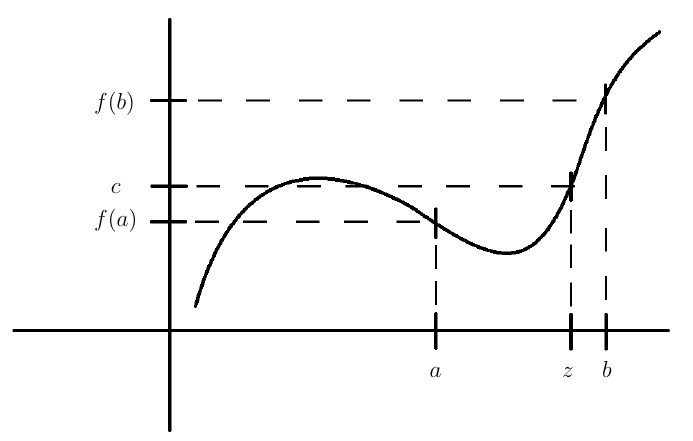
\includegraphics[width=\linewidth]{zwischenwertsatz.png}
 Wird häufig verwendet um zu zeigen, das eine Funktion einen gewissen Wert (z.B. Nullstelle) annimmt.
 \vspace{-4pt}
\end{mainbox}
Daraus folgt, dass ein Polynom mit ungeradem Grad mindestens eine Nullstelle in $\R$ besitzt.

\subsubsection{Kompaktes Intervall}
Ein Intervall $I \in \R$ ist kompakt, falls es von der Form $I = [a,b]$ mit $a \le b$ ist.
Dann ist Bild $f = f(I)$ ist auch ein kompaktes Intervall J = [min$f$, max$f$].

\begin{mainbox}{Min-Max-Satz}
  \vspace{-4pt}
 Sei $f: I = [a,b] \to \R$ stetig auf einem kompakten Intervall $I$. Dann gibt es $u, v \in I$ mit $f(u) \le f(x) \le f(v), \forall x \in I$. Insbesondere ist $f$ beschränkt.
 \vspace{-4pt}
\end{mainbox}

%\begin{subbox}{Stetigkeit der Verknüpfung}
 %Sei $f: D_1 \to D_2, g: D_2 \to \R$ und $x_0 \in D_1$. Falls $f$ in $x_0$ und $g$ in $f(x_0)$ stetig ist, dann ist $g \ocircle f: D_1 \to \R$ in $x_0$ stetig.
%\end{subbox}

\begin{mainbox}{Satz über die Umkehrabbildung}
  \vspace{-4pt}
 Sei $f: I \to \R$ stetig und streng monoton und sei $J = f(I) \subseteq \R$. Dann ist $f^{-1}: J \to I$ stetig und streng monoton.
 \vspace{-4pt}
\end{mainbox}

\begin{subbox}{Die reelle Exponentialfunktion}
  \vspace{-4pt}
  $\exp: \R \to \ ]0,+\infty[$ ist streng monoton wachsend, stetig und surjektiv. Auch die Umkehrfunktion $\ln: \ ]0,+\infty[ \to \R$ hat diese Eigenschaften.
  \vspace{-4pt}
\end{subbox}

\subsection{Funktionenfolgen}
Eine Funktionenfolge ist eine Abbildung $\N \to \{f: D \to \R \}$.
\begin{mainbox}{Punktweise Konvergenz}
  \vspace{-6pt}
  Die Funktionenfolge $(f_n)$ konvergiert punktweise gegen eine Funktion $f: D \to \R$ falls für alle $x \in D$ gilt, dass $\limn f_n(x) = f(x)$.
  \begin{itemize}
  \item $\forall x \in D, \forall \varepsilon>0, \exists N \in \N$ so dass $\forall n \geq \N, |f_n(x) -f(x)|<\varepsilon$
  \end{itemize}
  \vspace{-12pt}
\end{mainbox}

\begin{mainbox}{Gleichmässige Konvergenz}
  \vspace{-4pt}
 Die Folge $(f_n)$ konvergiert gleichmässig in $D$ gegen $f$ falls gilt:
 \begin{itemize}
  \item $\forall \varepsilon > 0 \ \exists N \ge 1$, so dass $\forall n \ge N, \ \forall x \in D: | f_n(x) - f(x) | \le \varepsilon$. 
  \item $\forall \varepsilon > 0 \ \exists N > 1$, so dass $\forall n, m \geq \N$ und $\forall x \in D: |f_n(x) - f_m(x)| < \varepsilon$.  
\end{itemize}
 Die Funktionenfolge $(g_n)$ ist gleichmässig konvergent, falls für alle $x\in D$ der Grenzwert $\limn g_n(x) = g(x)$ existiert und die Folge $(g_n)$ gleichmässig gegen $g$ konvergiert.
 \vspace{-12pt}
\end{mainbox}
Sei eine Funktionsfolge $(f_n)_{n \geq 0}$ stetig, dann ist die dazugehörige Funktion $f$ genau dann stetig, wenn $f_n$ gleichmässig konvergiert. Punktweise Konvergenz ist nicht ausreichend.
\begin{subbox}{}
  \vspace{-4pt}
  \textbf{Beispiel: }$f_n: [0, 1] \to \R \ x \to x^n$ konvergiert punktweise gegen $f(x) = \left\{
    \begin{array}{ll}
      0  & \mbox{ if } x < 1 \\
      1 & \mbox{ if } x = 1
    \end{array}
  \right.$
  \\$f_n: [0, 1] \to \R$ ist stetig $\forall n \in \N$
  aber die Grenzwertfunktion $f(x)$ ist nicht stetig.
  \vspace{-4pt}
\end{subbox}


Die Reihe $\sumk f_k(x)$ konvergiert gleichmässig, falls die durch $S_n(x) = \sum_{k=0}^n f_k(x)$ definierte Funktionenfolge gleichmässig konvergiert.

\begin{subbox}{}
  \vspace{-4pt}
 Sei $f_n$ eine Folge stetiger Funktionen. Ausserdem ist $|f_n(x)| \le c_n \quad \forall x \in D$ und $\sum_{n=0}^\infty c_n$ konvergiert. Dann konvergiert die Reihe $\sum_{n=0}^\infty f_n(x)$ gleichmässig und deren Grenzwert ist eine in $D$ stetige Funktion.
 \vspace{-4pt}
\end{subbox}

\subsection{Potenzreihen}
\begin{subbox}{Definition Potenzreihe}
\vspace{-4pt}
 Potenzreihen sind Reihen der Form $\sum_{n=0}^\infty a_n x^n$. Eine Potenzreihe mit Entwicklungspunkt $x_0$ wird als $\sum_{n=0}^\infty a_n(x-x_0)^n$ definiert.
 \vspace{-4pt}
\end{subbox}

\begin{mainbox}{Konvergenzradius}
  \vspace{-4pt}
 Der Konvergenzradius einer Potenzreihe um einen Entwicklungspunkt $x_0$ ist die grösste Zahl $r$, so dass die Potenzreihe für alle $x$ mit $|x - x_0| < r$ konvergiert. Falls die Reihe für alle $x$ konvergiert, ist der Konvergenzradius $r$ unendlich. Sonst:
 $$r = \limn \left| \frac{a_n}{a_{n+1}} \right| = \frac{1}{\limn\sup \sqrt[n]{|a_n|}} $$
 \vspace{-12pt}
\end{mainbox}
Die Potenzreihe $\sum_{k=0}^\infty a_n x^n$ konvergiert absolut für alle $|x| < r$ und divergiert für alle $|x| > r$. \textbf{Der Fall $|x| = r$ ist unklar und muss geprüft werden.}
\subsubsection{Definitionen per Potenzreihen}
\begin{align*}
\exp(x) &= \sumn \frac{x^n}{n!} & r &= \infty \\
\sin(x) &= \sumn (-1)^n \frac{x^{2n + 1}}{(2n + 1)!} & r &= \infty \\
\cos(x) &= \sumn (-1)^n \frac{x^{2n}}{(2n)!} & r &= \infty \\
\ln(x + 1) &= \sumk (-1)^{k+1} \frac{x^k}{k} & r &= 1
\end{align*}

Aus dem Leibnizkriterium und der Potenzreihenentwicklung von sin($x$) folgt $x - \frac{x^3}{6} \leq \sin (x) \leq x$ für $0 \leq x \leq \sqrt{6}$.

\subsection{Grenzwerte von Funktionen}
\begin{subbox}{Häufungspunkt}
  \vspace{-4pt}
 $x_0 \in \R$ ist ein Häufungspunkt der Menge D falls $\forall \delta > 0: (]x_0 - \delta, x_0 + \delta[ \backslash \{x_0\}) \cap D \ne \varnothing$.
 \vspace{-8pt}
\end{subbox}

\begin{mainbox}{Grenzwert - Funktionen}
  \vspace{-4pt}
 Wenn $f: D \to \R, x_0 \in \R$ ein Häufungspunkt von $D$ ist, dann ist $A \in \R$ der Grenzwert von $f(x)$ für $x \to x_0$ ($\lim_{x\to x_0} f(x) = A$), falls $\forall \varepsilon > 0 \ \exists \delta > 0$, so dass $\forall x \in D \cap (]x_0 - \delta, x_0 + \delta[ \backslash \{x_0\}): |f(x) - A| < \varepsilon$.
 \vspace{-4pt}
\end{mainbox}
Eine Funktion $f$ ist in $x_0$ stetig $\iff$ $\lim_{x \to x_0} f(x)$ existiert und gleich $f(x_0)$.
\\ \\
Die Stetigkeit einer abschnittweise definierten Funktion hängt auch vom Verhalten(links-/rechtsseitiger Grenzwert) an den Grenzen von Abschnittsintervallen ab.

\begin{subbox}{Satz von L'Hôpital}
  \vspace{-4pt}
  Seien $f,g$ stetig und differenzierbar auf $]a,b[$. Wenn $\lim_{x\to c} f(x) = \lim_{x \to c} g(x) = 0$ oder $\pm \infty$ und $g'(x) \ne 0 \ \forall x \in I \backslash \{c\}$, dann gilt $$\lim_{x\to c} \frac{f(x)}{g(x)} = \lim_{x\to c}\frac{f'(x)}{g'(x)}$$
  \vspace{-12pt}
\end{subbox}

Grenzwerte der Form $\infty^0$ und $1^\infty$ können meist mit $f(x)^{g(x)} = e^{g(x)\cdot \ln(f(x))}$ und dann Bernoulli (nur Exponenten betrachten da $e$ stetig) anwenden oder vereinfachen berechnet werden.

\begin{subbox}{Sandwichsatz für Grenzwerte}
  \vspace{-4pt}
  $D = \R \backslash \{0\}, f(x) = \frac{\sin (x)}{x}$
  Wir beweisen $\limxo f(x) = 1$ per Sandwichsatz:
  Wir haben schon gesehen, dass für $0 \leq x \leq \sqrt{6}$ $x - \frac{x^3}{3!} \leq \sin (x) \leq x$. Daraus folgt $1 - \frac{x^2}{3!} \leq \frac{\sin x}{x} \leq 1, \forall x \in ]0, \sqrt{6}[$.\\
  Da $1 - \frac{x^2}{3!}, 1 \to 1$ für $x \to 0$ gilt per Sandwichsatz $\frac{\sin(x)}{x} \to 1$.
  \vspace{-4pt}
\end{subbox}

\subsection{Beweisideen}%

\emph{Injektivität}
\begin{itemize}
	\item Zeigen, dass $f^{-1}$ surjektiv ist.
	\item Zeigen, dass gilt $y_1=y_2 \implies x_1=x_2$.
	\item Annehmen, dass es zwei verschiedene Punkte gibt, dann Widerspruch herbeiführen (Norm hilfreich?).
	\item Zeigen, dass die Ableitung $\neq 0$ ist, die Funktion also streng monoton wachsend/fallend.
\end{itemize}

\emph{Surjektivität}
\begin{itemize}
	\item Zeigen, dass gilt $\lim_{x\rightarrow\infty}f(x)=\infty$ und \\$\lim_{x\rightarrow-\infty}f(x)=-\infty$ 
	\item Zeigen, dass $f^{-1}$ keine Lücken im Definitionsbereich hat.
\end{itemize}

\subsubsection{Gerade/Ungerade}%


Für eine gerade Funktion gilt $f(x)=f(-x)$, sie ist symmetrisch zur Y-Achse.\\
Eine ungerade Funktion ist punktsymmetrisch zum Ursprung, es gilt also $f(-x)=-f(x)$.

\subsection{Algebraische und Analytische Eigenschaften}%


\begin{itemize}
	\item Jedes Vielfache einer geraden bzw. ungeraden Funktion ist wieder gerade bzw. ungerade.
	\item Die Summe zweier gerader Funktionen ist wieder gerade.
	\item Die Summe zweier ungerader Funktionen ist wieder ungerade.
	\item Das Produkt zweier gerader Funktionen ist wieder gerade.
	\item Das Produkt zweier ungerader Funktionen ist gerade.
	\item Das Produkt einer geraden und einer ungeraden Funktion ist ungerade.
	\item Der Quotient zweier gerader Funktionen ist wieder gerade.
	\item Der Quotient zweier ungerader Funktionen ist gerade.
	\item Der Quotient einer geraden und einer ungeraden Funktion ist ungerade.
	\item Die Komposition einer beliebigen Funktion mit einer geraden Funktion ist gerade.
	\item Die Komposition einer ungeraden Funktion mit einer ungeraden Funktion ist ungerade.
	\item Die Ableitung einer geraden differenzierbaren Funktion ist ungerade, die Ableitung einer ungeraden differenzierbaren Funktion gerade. 
	\item Das bestimmte Integral einer ungeraden stetigen Funktion ergibt $0$, wenn die Integrationsgrenzen symmetrisch um den Nullpunkt liegen.
\end{itemize}


\section{Ableitungen}
\subsection{Differenzierbarkeit}
\begin{mainbox}{Differenzierbar}
  \vspace{-4pt}
 $f$ ist \textbf{in $x_0$ differenzierbar}, falls der Grenzwert $$\lim_{h \to 0} \frac{f(x_0 + h) - f(x_0)}{h} = \lim_{x\to x_0} \frac{f(x) - f(x_0)}{x - x_0}$$ existiert. Wenn dies der Fall ist, wird der Grenzwert mit $f'(x_0)$ oder $\frac{d}{dx}f(x_0)$ bezeichnet. $f$ ist \textbf{differenzierbar}, falls $f$ für jedes $x_0 \in D$ differenzierbar ist.
 \vspace{-4pt}
\end{mainbox}
\begin{subbox}{Differenzierbarkeit nach Weierstrass}
  \vspace{-4pt}
  $f$ ist in $x_0$ differenzierbar $\iff$ 
 \begin{itemize}
  \item Es gibt $c \in \R$ und $r: D \to \R$ mit $f(x) = f(x_0) + c(x - x_0) + r(x) (x - x_0)$ und $r(x_0) = 0$, $r$ stetig in $x_0$. 
  \begin{itemize}
  \item Falls $f$ differenzierbar ist, dann ist $c = f'(x_0)$ und $r(x) = \frac{f(x) - f(x_0)}{x - x_0}$ eindeutig bestimmt.
  \end{itemize}
  \item Variation: Sei $\phi(x) = f'(x_0) + r(x)$. Dann gilt $f$ in $x_0$ differenzierbar, falls $f(x) = f(x_0) + \phi(x) (x-x_0), \ \forall x \in D$ und $\phi$ in $x_0$ stetig ist.
  Dann gilt $\phi(x_0) = f'(x_0)$.
  
 \end{itemize} 
 \vspace{-4pt}
\end{subbox}

\begin{subbox}{$f$ differenzierbar $\implies f$ stetig}
  \vspace{-4pt}
  Dies folgt aus der Varation der Differenzierbarkeit nach Weierstrass.
  \\\textit{Beweis:} Sei $x_0 \in D$ beliebig und $f$ differenzierbar.
  $\limxo f(x) = \limxo (f(x_0) + \phi(x)(x - x_0)) \overset{\phi(x) \text{ stetig}}{=} f(x_0) + \phi(x_0) \cdot \limxo(x - x_0) = f(x_0)$.
  \\ \\\textbf{Bmk:} Es gibt stetige Funktionen auf $\R$ die an keiner Stelle $x_0 \in \R$ differenzierbar sind.
  \\ Sei $g(x) = <x> := \min \{|x-m|\vert m \in \Z\}$ und dann ist $f(x) := \sumn \frac{g(10^nx)}{10^n}$ stetig auf $\R$ doch in keinem Punkt differenzierbar.
  \vspace{-4pt}
\end{subbox}

\begin{mainbox}{Höhere Ableitungen}
  \vspace{-8pt}
 \begin{enumerate}
  \item Für $n \ge 2$ ist $f$ n-mal differenzierbar in $D$ falls $f^{(n-1)}$ in $D$ differenzierbar ist. Dann ist $f^{(n)} = (f^{(n-1)})'$ die n-te Ableitung von $f$.
  \item $f$ ist n-mal stetig differenzierbar in $D$, falls sie n-mal differenzierbar und $f^{(n)}$ in $D$ stetig ist.
  \item $f$ ist in $D$ glatt, falls sie $\forall n \ge 1$ n-mal differenzierbar ist (``unendlich differenzierbar'').
 \end{enumerate}
 \vspace{-12pt}
\end{mainbox}
Glatte Funktionen: $\exp, \sin, \cos, \sinh, \cosh, \tanh, \ln,$\\ $ \arcsin, \arccos, \text{arccot}, \arctan$ und alle Polynome. $\tan$ ist auf $\R \backslash \{\pi/2 + k\pi\}$, $\cot$ auf $\R \backslash \{k\pi\}$ glatt.

\begin{subbox}{Höhere Ableitungen: Regeln}
  \vspace{-4pt}
  Sei $f, g$ n-mal differenzierbar. Dann sind $$(f + g), f \cdot g, f \circ g, \frac{f}{g}$$
  n-mal differenzierbar. ($g \neq 0$ für $\frac{f}{g}$)
  \begin{itemize}
  \item $(f \cdot g)^{(n)} = \sum_{k = 0}^{n} \binom{n}{k} f^{(k)} g^{(n-k)}$
  \end{itemize}
  \vspace{-10pt}
\end{subbox}

\subsection{Ableitungsregeln}

\begin{itemize}
  \item Linearität der Ableitung
  $$(\alpha \cdot f(x) + g(x))' = \alpha \cdot f'(x) + g'(x)$$
  \item Produktregel
  $$(f(x) \cdot g(x))' = f'(x) \cdot g(x) + f(x) \cdot g'(x)$$
  \item Quotientenregel
  $$\left(\frac{f(x)}{g(x)}\right)' = \frac{f'(x) \cdot g(x) - f(x) \cdot g'(x)}{g(x)^2}$$
  \item Kettenregel
  $$(f(g(x)))' = g'(x) \cdot f'(g(x))$$
  \item Potenzregel
  $$(c \cdot x^a)' = c \cdot a \cdot x^{a - 1}$$
  \item Umkehrregel
  $$(f^{-1})' (x) = \frac{1}{f'(f^{-1} (x))}, f'(f^{-1} (x)) \neq 0$$
  \\ $f$ muss bijektiv und differenzierbar sein. $f^{-1}$ muss in $x$ differenzierbar sein. 
\end{itemize}

\subsection{Implikationen der Ableitung}
\begin{enumerate}
  \item $f$ besitzt ein lokales Minimum in $x_0$, wenn $f'(x_0) = 0$ und $f''(x_0) > 0$ oder falls das Vorzeichen von $f'$ um $x_0$ von $-$ zu $+$ wechselt.
  \item $f$ besitzt ein lokales Maximum in $x_0$, wenn $f'(x_0) = 0$ und $f''(x_0) < 0$ oder falls das Vorzeichen von $f'$ um $x_0$ von $+$ zu $-$ wechselt.
  \item $f$ besitzt ein lokales Extremum in $x_0$, wenn $f'(x_0) = 0$ und $f''(x_0) \ne 0$.
   \\ \textbf{Wenn man den Vorzeichenwechsel benutzen will, um auf ein Extremum zu schliessen, dann muss $f'$ stetig sein. }
  \item Wenn $f'(x_0) = 0$ und $f''(x_0) = 0$, ist $x_0$ nicht unbedingt ein Sattelpunkt. 
  \\Als Gegenbeispiel siehe $f(x)= x^4$, $f''(0) = 0$ aber $x = 0$ ist ein Minimum von $f$.
  \item $f$ besitzt einen Wendepunkt in $x_0$, wenn $f''(x_0) = 0$.
  \item $f$ ist in $x_0$ konvex, wenn $f''(x_0) \ge 0$.
  \item $f$ ist in $x_0$ konkav, wenn $f''(x_0) \le 0$.
\end{enumerate}

\subsection{Sätze zur Ableitung}
\begin{subbox}{Satz von Rolle}
  \vspace{-4pt}
 Sei $f: [a,b] \to \R$ stetig und in $]a,b[$ differenzierbar. Wenn $f(a) = f(b)$, dann gibt es mindestens ein $\xi \in ]a,b[$ mit $f'(\xi) = 0$.
 \vspace{-4pt}
\end{subbox}
\begin{mainbox}{Mittelwertsatz (Lagrange)}
  \vspace{-4pt}
 Sei $f: [a,b] \to \R$ stetig und in $]a,b[$ differenzierbar. Dann gibt es (mindestens ein) $\xi \in ]a,b[$ mit $f(b) - f(a) = f'(\xi)(b-a)$.
 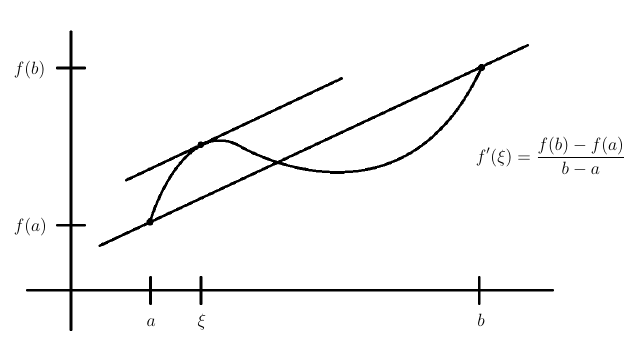
\includegraphics[width=\linewidth]{mittelwertsatz.png}
 \vspace{-4pt}
\end{mainbox}

\subsection{Taylorreihen}
Taylorreihen sind ein Weg, glatte Funktionen als Potenzreihen anzunähern.

\begin{mainbox}{Definition: Taylor-Polynom}
  \vspace{-4pt}
  Sei $f : [a, b] \to \R$ stetig und in $]a, b[$ (n+1)-mal differenzierbar. 
 \\Das n-te Talyor-Polynom $T_n f(x; a)$ an einer Entwicklungsstelle $a$ ist definiert als:
 $$T_n f(x; a) := \sum_{k=0}^{n} \frac{f^{(k)} (a)}{k!} \cdot (x - a)^k$$ 
 $ = f(a) + f'(a) \cdot (x-a) + \frac{f''(a)}{2} \cdot (x - a)^2 + \ldots$
 \\ \\Da eine Abschätzung mit dem Taylor-Polynom im allgemeinen Fall einen gewissen Fehler hat, definieren wir das Restglied $R_n(f, x, a)$.
 \\ \\
 Für jedes $a < x <b$ gibt es ein $\xi \in ]a, x[$ mit:
 $$f(x) = T_n f(x; a) + \frac{f^{(n+1)}(\xi)}{(n+1)!}(x - a)^{n+1}$$
 Wobei $$R_n(f, x, a) := \frac{f^{(n+1)}(\xi)}{(n+1)!}(x - a)^{n+1}$$
\end{mainbox}

\begin{subbox}{Fehlerabschätzung des Taylor-Polynoms}
  Sei $\alpha \in \R$ der Fehler des Taylorpolynoms.
  \begin{align*}
    |\alpha| &\leq \sup_{\xi \in [a, x]} |R_n(f, x, a)|\\
             &= \sup_{\xi \in [a, x]} \bigg|\frac{f^{(n+1)}(\xi)}{(n+1)!}(x-a)^{(n+1)}\bigg|
  \end{align*}
\end{subbox}

\begin{mainbox}{Taylorreihe}
  \vspace{-4pt}
 Die unendliche Reihe
 $$Tf(x;a) := T_\infty = \sumn \frac{f^{(n)}(a)}{n!} \cdot (x-a)^n$$
 wird Taylorreihe von $f$ an Stelle $a$ genannt.
 \\(Dafür muss die Funktion $f$ glatt sein.)
 \vspace{-4pt}
\end{mainbox}

\begin{subbox}{Differenzierbarkeit von Potenzreihen}
  \vspace{-4pt}
  Funktionen die durch Potenzreihen gegeben sind, sind als Polynome gliedweise differenzierbar. Innerhalb ihres Konvergenzbereichs sind sie glatte Funktionen.
  \\Sei $f(x) = \sumn \frac{f^{(n)}(a)}{n!}\cdot(x-a)^n$ die Taylorreihe der Funktion $f$.
  \\Dann kann man die $j$-te Ableitung wie folgt ausdrücken:
  $$f^{(j)}(x) = \sum_{n = j}^{\infty} \frac{f^{(n)}(a)}{n!} \cdot \frac{n!}{(n-j)!} \cdot (x - a)^{(n-j)}$$
  Für eine allgemeine Potenzreihe gilt:
  $$f(x) = \sum_{k = 0}^{\infty} c_k\cdot(x-x_0)^k$$ 
  $$ f^{(j)}(x) = \sum_{k = j}^{\infty} c_k \frac{k!}{(k-j)!}(x-x_0)^{k-j}$$
  \vspace{-12pt}
\end{subbox}

Beispiele Taylorreihen ($a = 0$):
\begin{itemize}
 \item $\sin(x) = \sumn (-1)^n \cdot \frac{x^{2n+1}}{(2n+1)!}$
 \item $\cos(x) = \sumn (-1)^n \cdot \frac{x^{2n}}{(2n)!}$
 \item $e^x = \sumn \frac{x^n}{n!}$
 \item $e^{-x} = \sumn (-1)^n \cdot \frac{x^n}{n!}$
 \item $\sinh(x) = \sumn \frac{x^{2n+1}}{(2n+1)!}$
 \item $\cosh(x) = \sumn \frac{x^{2n}}{(2n)!}$
\end{itemize}

\subsection{Länge einer Kurve}
Für eine Kurve $p(t) = (x(t), y(t))$ in der $xy$-Ebene gilt 
$$L = \int_a^b \sqrt{x'(t)^2+ y'(t)^2} \text{ d}t$$

\section{Integrale}

\subsection{Riemann-Integral}

\begin{subbox}{Definition: Partition}
  \vspace{-4pt}
 Eine Partition von $I = [a, b]$ ist eine endliche Teilmenge $P = \{a = x_0, x_1, x_2, ..., x_n = b\} \subsetneq I$, wobei $x_0 < x_1 < ... < x_n$ und $\{a,b\} \subseteq P$. (``Aufteilung'')
 \\Wir bezeichnen $\delta_i := x_i - x_{i-1}, \forall i \geq 1 $ (Länge des Teilintervalls)
 \\Die \textbf{Feinheit der Zerlegung} ist definiert als $\delta(P) := \max_{1 \leq i \leq n} \delta_i$.
 \\Wir definieren $\mathcal{P}(I)$ als die Menge aller Partitionen von $I$.
 \\$\mathcal{P}_{\delta}(I) := \{P \in \mathcal{P}(I) \vert \delta(P) \leq \delta\}$
 \vspace{-6pt}
\end{subbox}


\begin{mainbox}{Definition: Riemann-Summe}
  \vspace{-4pt}
  Sei $\xi_i \in I_i$ zwischen den Stützstellen: \\$x_{i-1} \leq \xi_i \leq x_i$, 
  $\xi = \{\xi_1, \xi_2, ..., \xi_n \}$
 $$S(f, P, \xi) := \sum_{i=1}^n f(\xi_i) \cdot (x_i - x_{i-1})$$
 \vspace{-12pt}
\end{mainbox}

\begin{subbox}{Ober- und Untersumme}
  \vspace{-4pt}
  Sei $f: [a, b] \to \R$ eine beschränkte Funktion, d.h. $\exists M \geq 0$ mit $|f(x)| \leq M, \forall x \in [a,b]$
\\ Obersumme: $$\overline{S}(f,P) := \sum_{i = 1}^{n}\sup_{\xi_i \in I_i} f(\xi_i) \cdot \delta_i$$ 
 Untersumme: $$\underline{S}(f,P) := \sum_{i = 1}^{n}\inf_{\xi_i \in I_i} f(\xi_i) \cdot \delta_i$$
 \textbf{Bmk:}
 \\$-M \cdot (b-a) \leq \underline{S}(f,P) \leq \overline{S}(f,P) \leq M \cdot (b-a)$
 \vspace{-4pt}
\end{subbox}

Seien $P, Q$ Partitionen des gleichen Intervalls.
\begin{itemize}
  \item Eine Vereinigung von zwei Partitionen ist wieder eine Partition.
  \item Eine Partition $P$ ist eine Verfeinerung einer Partition $Q$, falls $Q \subset P$.
  \item $P \cup Q$ ist immer eine Verfeinerung von $P$ und $Q$.
  \item $P \subset Q \implies \underline{S}(f, P) \leq \underline{S}(f, Q) \leq \overline{S}(f, Q) \leq \overline{S}(f, P)$
  \item Für $P, Q$ beliebig gilt: $\underline{S}(f, P) \leq \overline{S}(f, Q)$
  \\Insbesondere $$\sup_{P \in \mathcal{P}(I)} \underline{S}(f, P) \leq \inf_{P \in \mathcal{P}(I)} \overline{S}(f, P)$$
\end{itemize}


\begin{mainbox}{Riemann-integrierbar}
  \vspace{-4pt}
  Wir definieren das untere Riemann Integral 
  $$\underline{S}(f):= \sup_{P \in \mathcal{P}(I)} \underline{S}(f, P)$$   
  und das obere Riemann Integral von $f$ 
  $$\overline{S}(f) := \inf_{P \in \mathcal{P}(I)} \overline{S}(f, P)$$
 \\Eine beschränkte Funktion $f:[a,b] \to \R$ ist Riemann-integrierbar, falls $\underline{S}(f) = \overline{S}(f)$. Dann ist 
 $$A := \int_a^b f(x)\dx = \underline{S}(f) = \overline{S}(f), A \in \R$$%\limn \sum_{n = 1}^{\infty} f(\xi_i)\delta_i
 \vspace{-12pt}
\end{mainbox}

\subsection{Integrierbarkeit zeigen}

\begin{mainbox}{Integrierbarkeitskriterien}
  \vspace{-4pt}
  Sei $f: [a, b] \to \R$ beschränkt und $A = \int_{a}^{b} f(x)dx$ falls $f$ integrierbar.
  \\$f$ integrierbar 
  \\$\iff$\\
  $\forall \varepsilon > 0, \exists P \in \mathcal{P}(I)$ mit $\overline{S}(f, P) - \underline{S}(f, P) < \varepsilon$
  \\$\iff$\\ 
  $\forall \varepsilon > 0, \exists \delta > 0$, so dass $\overline{S}(f, P) - \underline{S}(f, P) < \varepsilon, \forall P \in \mathcal{P}_{\delta}(I)$ 
  \\$\iff$\\
  $\forall \varepsilon > 0, \exists \delta > 0$, so dass $\forall P \in \mathcal{P}_{\delta}(I)$ und $\xi_1, ...,\xi_n$ mit $\xi \in [x_{i-1},x_i]$
  \\$|A - S(f, P, \xi)| < \varepsilon$ 
  \\$\iff$\\
  $lim_{\delta(P) \to 0} S(f, P, \xi)$ existiert. 
  (Dann wäre $lim_{\delta(P) \to 0} S(f, P, \xi) = A$)
  \vspace{-4pt}
\end{mainbox}

\begin{subbox}{Gleichmässige Stetigkeit}
  \vspace{-4pt}
  Eine Funktion $f: D \to \R$ ist \textbf{gleichmässig stetig}, falls $\forall \varepsilon > 0, \exists \delta > 0 \ \forall x, y \in D:$
  \\$|x - y| < \delta \implies |f(x) - f(y)| < \varepsilon$
  \\(Das $\delta$ hängt nur vom $\varepsilon$ ab)
  \vspace{-4pt}
\end{subbox}

  Die Funktion $f: \R \to \R, f(x) = x^2$ ist auf $\R$ stetig aber nicht gleichmässig stetig.
\begin{subbox}{Satz von Heine}
  \vspace{-4pt}
  Sei $f: [a,b] \to \R$ stetig in dem \textbf{kompakten Intervall} $[a,b]$. Dann ist $f$ in $[a,b]$ gleichmässig stetig.
  \vspace{-4pt}
\end{subbox}

\begin{mainbox}{}
  \vspace{-4pt}
  Sei $f: [a, b] \to \R$ stetig. Dann ist $f$ integrierbar.
  \vspace{-4pt}
\end{mainbox}

\begin{itemize}
 \item $f$ stetig in $[a,b] \implies f$ integrierbar über $[a,b]$
 \item $f$ monoton in $[a,b] \implies f$ integrierbar über $[a,b]$
 \item Wenn $f,g$ beschränkt und integrierbar sind, dann sind
 $$f+g, \lambda \cdot f, f \cdot g, |f|, \max(f,g), \min(f,g), \frac{f}{g}$$ integrierbar
 \item Jedes Polynom ist integrierbar, auch $\frac{P(x)}{Q(x)}$ falls $P(x), Q(x)$ auf $[a,b]$ definiert sind und $Q(X)$ in $[a,b]$ keine Nullstellen besitzt
\end{itemize}


\subsection{Sätze \& Ungleichungen}
\begin{itemize}
 \item $f(x) \le g(x), \forall x \in [a,b] \rightarrow \int_a^b f(x) \dx \le \int_a^b g(x) \dx$
 \item $\left|\int_a^b f(x) \dx\right| \le \int_a^b |f(x)| \dx$
 \item $\left|\int_a^b f(x) g(x) \dx \right| \le \sqrt{\int_a^b f^2(x) \dx} \sqrt{\int_a^b g^2(x) \dx}$
\end{itemize}

\begin{mainbox}{Mittelwertsatz}
  \vspace{-4pt}
 Wenn $f: [a,b] \to \R$ stetig ist, dann gibt es $\xi \in [a,b]$ mit $\int_a^b f(x) \dx = f(\xi) (b-a)$.
 \vspace{-4pt}
\end{mainbox}
Daraus folgt auch, dass wenn $f,g: [a,b] \to \R$ wobei $f$ stetig, $g$ beschränkt und integrierbar mit $g(x) \ge 0, \forall x \in [a,b]$ ist, dann gibt es $\xi \in [a,b]$ mit $\int_a^b f(x)g(x) \dx = f(\xi) \int_a^b g(x) \dx$.

\subsection{Stammfunktionen}
\begin{subbox}{Definition: Stammfunktion}
  \vspace{-4pt}
 Eine Funktion $F: [a,b] \to \R$ heisst Stammfunktion von $f$, falls $F$ (stetig) differenzierbar in $[a,b]$ ist und $F' = f$ in $[a,b]$ gilt.
 \vspace{-4pt}
\end{subbox}
``$f$ integrierbar'' impliziert \textit{nicht}, dass eine Stammfunktion existiert. Beispiel:
$$
 f(x) = \begin{cases}
        0, & \text{für } x \le 0 \\
        1, & \text{für } x > 0
        \end{cases}
$$

\begin{mainbox}{Hauptsatz der Integral- und Differentialrechnung}
  \vspace{-4pt}
  Sei $a<b$ und $f: [a,b] \to \R$ stetig. Die Funktion 
 $$F(x) = \int_a^x f(t) \text{ d}t, \ a \le x \le b$$
 ist in $[a,b]$ stetig differenzierbar und $F'(x) = f(x) \ \forall x \in [a,b]$.
 \vspace{-4pt}
\end{mainbox}

\begin{mainbox}{Fundamentalsatz der Analysis}
  \vspace{-4pt}
  Sei $f: [a,b] \to \R$ stetig. Dann gibt es eine Stammfunktion $F$ von $f$, die bis auf eine additive Konstante eindeutig bestimmt
  ist und es gilt: $$\int_a^b f(x)dx = F(b) - F(a)$$
  \vspace{-4pt}
\end{mainbox}

\subsection{Integrationsregeln}
\begin{subbox}{Erweiterung der Definition eines Integrals}
  \vspace{-4pt}
  Wir erweitern die Definition, so dass $$\int_a^b f(x)\dx := - \int_b^a f(x)dx$$ und $$\int_a^a f(x)dx := 0$$
  \vspace{-8pt}
\end{subbox}

\begin{subbox}{Linearität}
 \vspace{-12pt}
 $$\int u\cdot f(x) + v \cdot g(x) \dx = u \int f(x) \dx + v \int g(x) \dx$$
 \vspace{-12pt}
\end{subbox}
\begin{subbox}{Gebietsadditivität}
 \vspace{-12pt}
 $$\int_a^b f(x) \dx = \int_a^c f(x) \dx + \int_c^b f(x) \dx, \ c \in [a,b]$$
 \vspace{-12pt}
\end{subbox}
\begin{mainbox}{Partielle Integration}
 \vspace{-12pt}
 $$\int f'(x) g(x) \dx = f(x)g(x) - \int f(x) g'(x) \dx$$
 \vspace{-12pt}
\end{mainbox}
\begin{itemize}
 \item Grundsätzlich gilt: Polynome ableiten ($g(x)$), wo das Integral periodisch ist ($\sin, \cos, e^x$,...) integrieren ($f'(x)$)
 \item Teils ist es nötig, mit $1$ zu multiplizieren, um partielle Integration anwenden zu können (z.B. im Fall von $\int \log(x) \dx$)
 \item Muss eventuell mehrmals angewendet werden
\end{itemize}
\begin{mainbox}{Substitution}
  \vspace{-12pt}
 Um $\int_a^b f(g(x)) \dx$ zu berechnen: Ersetze $g(x)$ durch $u$ und integriere $\int_{g(a)}^{g(b)} f(u) \frac{\text{d}u}{g'(x)}$.
 \vspace{-12pt}
\end{mainbox}
\begin{itemize}
 \item $g'(x)$ muss sich irgendwie herauskürzen, sonst nutzlos.
 \item Grenzen substituieren nicht vergessen.
 \item Alternativ kann auch das unbestimmte Integral berechnet werden und dann $u$ wieder durch $x$ substituiert werden.
\end{itemize}

\begin{mainbox}{Partialbruchzerlegung}
  \vspace{-4pt}
 Seien $p(x), q(x)$ zwei Polynome. $\int \frac{p(x)}{q(x)}$ wird wie folgend berechnet:
 \begin{enumerate}
  \item Falls $\deg(p) \ge \deg(q)$, führe eine Polynomdivision durch. Dies führt zum Integral $\int a(x) + \frac{r(x)}{q(x)}$.
  \item Berechne die Nullstellen von $q(x)$.
  \item Pro Nullstelle: Einen Partialbruch erstellen.
  \begin{itemize}[left=0pt]
   \item Einfach, reell: $x_1 \to \frac{A}{x - x_1}$
   \item $n$-fach, reell: $x_1 \to \frac{A_1}{x - x_1} + \ldots + \frac{A_r}{(x-x_1)^r}$ 
   \item Einfach, komplex: $x^2 + px + q \to \frac{Ax + B} {x^2 + px + q}$
   \item $n$-fach, komplex: $x^2 + px + q \to \frac{A_1x+b_1}{x^2+px+q} + \ldots$
  \end{itemize}
  \item Parameter $A_1, \ldots, A_n$ (bzw. $B_1, \ldots, B_n$) bestimmen. ($x$ jeweils gleich Nullstelle setzen, umformen und lösen).

 \end{enumerate}
 \vspace{-10pt}
\end{mainbox}

\subsection{Integration konvergenter Reihen}

\begin{mainbox}{Funktionsfolge integrieren}
  \vspace{-4pt}
  Sei $f_n: [a, b] \to \R$ eine Folge von beschränkten, integrierbaren Funktionen, die gleichmässig gegen $f: [a,b] \to \R$ konvergiert.
  Dann ist $f$ beschränkt und integrierbar:
  $$\limn \int_a^b f_n(x)dx =\int_a^b \left(\limn f_n(x)\right)dx$$
  (ohne gleichmässige Konvergenz dürfte man den lim und das Integral nicht tauschen!)
  Sei $\sumn f_n$ auf $[a, b]$ gleichmässig konvergent. Dann gilt:
  $$\sumn \int_a^b f_n(x)dx = \int_a^b \left(\sumn f_n(x)\right) dx$$
  \vspace{-12pt}
\end{mainbox}

\begin{mainbox}{Integration von Potenzreihen}
  \vspace{-4pt}
  Sei $f(x) := \sum_{k = 0}^{\infty} c_k x^k$ eine Potenzreihe mit positivem Konvergenzradius $\rho > 0$. Dann ist $f$ auf $[-r,r]$ integrierbar $\forall r \in [0, \rho[$ und es gilt:
  $\int_a^b f(t)dt = \sum_{k = 0}^{\infty} c_k \frac{x^{k+1}}{k+1}, \forall x \in ]-\rho, \rho[$
  \vspace{-6pt}
\end{mainbox}
\textbf{Bmk:} Im Allg. kann man Potenzreihen in ihrem Konvergenzbereich termweise differenzieren und integrieren.

\subsection{Euler-McLaurin-Formel}
Die Formel hilft Summen wie $1^l + 2^l + 3^l + ... + n^l$ abzuschätzen.
Für die Formel brauchen wir die Bernoulli-Polynome $B_n(x)$, sowie die Bernoulli-Zahlen $B_n(0)$.
Wir brauchen dafür Polynome, welche durch die folgenden Eigenschaften bestimmt sind:

\begin{enumerate}
  \item $P'_k = P_{k-1}, k > 1$
  \item $\int_0^1 P_k(x)\dx = 0, \forall k \geq 1$
\end{enumerate}

Für das $k$-te Bernoulli-Polynom gilt: $B_k(x) = k!P_k(x)$. Wir definieren weiter $B_0=1$ und alle anderen Bernoulli-Zahlen rekursiv: $B_{k-1} = \sum_{i=0}^{k-1}{k \choose i}B_i = 0$.

Somit erhalten wir für das Bernoulli-Polynom folgende Definition: $$B_k(x) = \sum_{i=0}^{k}{k \choose i}B_ix^{k-i}$$

Hier ein paar Bernoulli-Polynome: $B_0(x) = 1$, $B_1(x) = x - \frac{1}{2}$, $B_2(x) = x^2 - x + \frac{1}{6}$. Nun definieren wir noch: $$\tilde{B}_k(x) = \begin{cases}
  B_k(x) & \forall x: 0 \leq x < 1 \\
  B_k(x-n) & \forall x: n \leq x < n + 1
\end{cases}$$

\begin{mainbox}{Euler-McLaurin-Summationsformel}
  \vspace{-4pt}
  Sei $f: [0, n] \to \R$ $k$-mal stetig differenzierbar. Dann gilt: \\
  Für $k = 1$:
  \begin{align*}
  \sum_{i = 1}^n f(i) = \int_0^n f(x) \dx + \frac{1}{2}(f(n) - f(0)) \\ + \int_0^n \tilde{B}_1(x)f'(x)\dx
  \end{align*}
  Für $k>1$:
  \begin{align*}
  \sum_{i = 1}^n f(i) = \int_0^n f(x) \dx + \frac{1}{2}(f(n) - f(0))+ \\
  \sum_{j = 2}^k \frac{(-1)^j B_j}{j!}(f^{(j-1)}(n) + f^{(j-1)}(0)) + \tilde{R}_k
  \end{align*}
  
  wobei
  $$ \tilde{R}_k = \frac{(-1)^{k-1}}{k!} \int_0^n \tilde{B}_k(x)f^{(k)}(x)\dx$$
  \vspace{-12pt}
\end{mainbox}

\begin{subbox}{Beispiel für Euler-McLaurin}
  \vspace{-12pt}
  $$1^l + 2^l + 3^l + ... + n^l \text{ wobei } l \geq 1, l \in \mathbb{N}$$
  Angewandt auf $f(x) = x^l$ und $k = l + 1$ folgt für alle $l \geq 1$:
  $$1^l + 2^l + 3^l + ... + n^l = \frac{1}{l + 1} \sum_{j = 0}^l (-1)^j B_j {l + 1 \choose j} n^{l+1-j}$$
  \vspace{-8pt}
\end{subbox}

\subsection{Gamma-Funktion}
Die Gamma-Funktion wird gebraucht, um die Funktion $n \mapsto (n-1)!$ zu interpolieren. Für $s > 0$ definieren wir: $$\Gamma(s) := \int_0^\infty e^{-x}x^{s-1}\dx = (s-1)!$$
Die Gamma-Funktion konvergiert für alle $s > 0$ und hat folgende weiter Eingeschaften:
\begin{enumerate}
  \item $\Gamma(1) = 1$
  \item $\Gamma(s + 1) = s \Gamma(s)$
  \item $\Gamma$ ist logarithmisch konvex, d.h.: $$\Gamma(\lambda x + (2 - \lambda)y) \leq \Gamma(x)^\lambda \Gamma(y)^{1 - \lambda}$$ für alle $x, y > 0$ und $0 \leq \lambda \leq 1$
\end{enumerate}
Die Gamma-Funktion ist die einzige Funktion $]0, \infty[ \to ]0, \infty[$, die $(1), (2)$ und $(3)$ erfüllt. Zudem gilt: $$\Gamma(x) = \limn \frac{n!n^x}{x(x+1)...(x+n)} \ \ \ \forall x > 0$$

\subsection{Stirling'sche Formel}
Die Stirling'sche Formel ist eine Abschätzung der Fakultät. Mit der Euler-McLaurin-Formel kombiniert folgt
$$n! = \frac{\sqrt{2\pi n} \cdot n^n}{e^n} \cdot \exp(\frac{1}{12n}+R_3(n))$$
wobei $|R_3(n)| \le \frac{\sqrt{3}}{216}\cdot\frac{1}{n^2} \ \forall n \ge 1$

\subsection{Uneigentliche Integrale}
\begin{subbox}{Definition: Uneigentliches Integral}
  \vspace{-4pt}
 Sei $f(x): \ [ a,\infty [ \to \R$ beschränkt und integrierbar auf $[a,b] $ mit $\forall b > a$ . Falls $\lim_{b\to\infty} \int_a^b f(x) \dx$ existiert, ist $\int_a^\infty f(x) \dx$ der Grenzwert und $f$ ist auf $[a, \infty[$ integrierbar.
 \vspace{-4pt}
\end{subbox}
Diese Definition gilt auch für $f(x) : \ ]-\infty,b] \to \R$, wobei $\int_{-\infty}^b f(x) \dx $ dann $ \lim_{a\to-\infty} \int_a^b f(x) \dx$ ist.

\begin{mainbox}{}
  \vspace{-4pt}
Falls $f: ]a,b] \to \R$ auf $]a, b]$ nicht beschränkt ist, aber auf jedem Intervall $[a+\varepsilon, b], \varepsilon > 0$, beschränkt und integrierbar ist, ist $f$ auf $]a,b]$ integrierbar falls
$lim_{\varepsilon \to 0^+} \int_{a+\varepsilon}^b f(x) dx$ existiert; in diesem Fall wird dieser Grenzwert mit $\int_a^b f(x)dx$ bezeichnet.
  \vspace{-4pt}
\end{mainbox}

\begin{mainbox}{Majoranten-/ Minorantenkriterium}
  \vspace{-4pt}
Sei $f: [a, \infty[ \to \R$ beschränkt, integrierbar auf $[a, b], \forall b > a$.
\begin{enumerate}
  \item $|f(x)| \leq g(x) ,\forall x \geq a$ und $g$ auf $[a, \infty[$ integrierbar
  \\$\implies$ $f$ auf $[a, \infty[$ integrierbar
  \item $0 \leq g(x) \leq f(x)$ und $\int_a^{\infty}g(x)dx$ divergiert
  \\$\implies$ $\int_a^{\infty}f(x)dx$ divergiert
\end{enumerate}
\vspace{-12pt}
\end{mainbox}



\begin{subbox}{McLaurin-Satz (Integraltest für Reihen)}
  \vspace{-4pt}
Sei $f: \ [1, \infty[ \ \to [0, \infty[$ monoton fallend. Dann konvergiert $\sum_{n=1}^\infty f(n)$ genau, wenn $\int_1^\infty f(x) \dx$ konvergiert.
In diesem Fall gilt: $0 \leq \sum_{n=1}^\infty f(n) - \int_1^\infty f(x) \dx \leq f(1)$
  \vspace{-4pt}
\end{subbox}

\subsection{Unbestimmte Integrale}
Sei $f: I \to \R$ auf dem Intervall $I \subseteq \R$ definiert. Wenn $f$ stetig ist, gibt es eine Stammfunktion $F$. Wir schreiben dann

$$\int f(x) \dx = F(x) + C$$

Das unbestimmte Integral ist die Umkehroperation der Ableitung.

\section{Trigonometrie}

Die Kreiszahl $\pi :=$ Inf$\{t > 0| \sin t = 0\}$. Beweisidee: $\sin x > 0, \forall x \in ]0, 2]$ und $\sin 4 < 0$. Da $\sin x$ stetig ist, gibt es per Zwischenwertsatz mindestens ein $x \in ]2, 4[$ so dass $\sin x = 0$.
\subsection{Hyperbelfunktionen}
\begin{itemize}
  \item $\cosh x := \frac{e^x + e^{-x}}{2} : \R \to [1, \infty]$
  \item $\sinh x := \frac{e^x - e^{-x}}{2} : \R \to \R$
  \item $\tanh x := \frac{e^x - e^{-x}}{e^x + e^{-x}}$
\end{itemize}

\subsection{Regeln}
\subsubsection{Periodizität}
\begin{itemize}
 \item $\sin(\alpha + 2 \pi) = \sin(\alpha) \quad \cos(\alpha + 2 \pi) = \cos(\alpha)$
 \item $\tan(\alpha + \pi) = \tan(\alpha) \quad \cot(\alpha + \pi) = \cot(\alpha)$
\end{itemize}

\subsubsection{Parität}
\begin{itemize}
 \item $\sin(-\alpha) = - \sin(\alpha) \quad \cos(-\alpha) = \cos(\alpha)$
 \item $\tan(-\alpha) = - \tan(\alpha) \quad \cot(-\alpha) = - \cot(\alpha)$
\end{itemize}

\subsubsection{Ergänzung}
\begin{itemize}
 \item $\sin(\pi - \alpha) = \sin(\alpha) \quad \cos(\pi - \alpha) = - \cos(\alpha)$
 \item $\tan(\pi - \alpha) = -\tan(\alpha) \quad \cot(\pi - \alpha) = - \cot(\alpha)$
\end{itemize}


\subsubsection{Komplemente}
\begin{itemize}
 \item $\sin(\pi/2 - \alpha) = \cos(\alpha) \quad \cos(\pi/2 - \alpha) = \sin(\alpha)$
 \item $\tan(\pi/2 - \alpha) = -\tan(\alpha) \quad \cot(\pi/2 - \alpha) = -\cot(\alpha)$
\end{itemize}

\subsubsection{Doppelwinkel}
\begin{itemize}
 \item $\sin(2\alpha) = 2 \sin(\alpha) \cos(\alpha)$
 \item $\cos(2\alpha) = \cos^2(\alpha) - \sin^2(\alpha) = 1 - 2 \sin^2(\alpha)$
 \item $\tan(2\alpha) = \frac{2\tan(\alpha)}{1 - \tan^2(\alpha)}$
\end{itemize}

\subsubsection{Addition}
\begin{itemize}
 \item $\sin(\alpha + \beta) = \sin(\alpha) \cos(\beta) + \cos(\alpha) \sin(\beta)$
 \item $\cos(\alpha + \beta) = \cos(\alpha) \cos(\beta) - \sin(\alpha) \sin(\beta)$
 \item $\tan(\alpha + \beta) = \frac{\tan(\alpha) + \tan(\beta)}{1 - \tan(\alpha) \tan(\beta)}$
\end{itemize}

\subsubsection{Subtraktion}
\begin{itemize}
 \item $\sin(\alpha - \beta) = \sin(\alpha) \cos(\beta) - \cos(\alpha)\sin(\beta)$
 \item $\cos(\alpha - \beta) = \cos(\alpha) \cos(\beta) + \sin(\alpha)\sin(\beta)$
 \item $\tan(\alpha - \beta) = \frac{\tan(\alpha) - \tan(\beta)}{1+\tan(\alpha) \tan(\beta)}$
\end{itemize}

\subsubsection{Multiplikation}
\begin{itemize}
 \item $\sin(\alpha) \sin(\beta) = -\frac{\cos(\alpha + \beta) - \cos(\alpha - \beta)}{2}$
 \item $\cos(\alpha) \cos(\beta) =  \frac{\cos(\alpha + \beta) + \cos(\alpha - \beta)}{2}$
 \item $\sin(\alpha) \cos(\beta) =  \frac{\sin(\alpha + \beta) + \sin(\alpha - \beta)}{2}$
\end{itemize}

\subsubsection{Potenzen}
\begin{itemize}
 \item $\sin^2(\alpha) = \frac{1}{2}(1-\cos(2\alpha))$
 \item $\cos^2(\alpha) = \frac{1}{2}(1+\cos(2\alpha))$
 \item $\tan^2(\alpha) = \frac{1-\cos(2\alpha)}{1+\cos(2\alpha)}$
\end{itemize}

\subsubsection{Diverse}

\begin{itemize}
 \item $\sin^2(\alpha) + \cos^2(\alpha) = 1$
 \item $\cosh^2(\alpha) - \sinh^2(\alpha) = 1$
 \item $\sin(z) = \frac{e^{iz} - e^{-iz}}{2}$ und $\cos(z) = \frac{e^{iz} + e^{-iz}}{2}$
 \\ \\In der Serie 8 wurde gezeigt, dass:
 \item $\sin x - \sin y = 2\sin\left(\frac{x-y}{2}\right)\cos\left(\frac{x+y}{2}\right)$
 \item $\cos x -\cos y = -2\sin\left(\frac{x-y}{2}\right)\sin\left(\frac{x+y}{2}\right)$
\end{itemize}


\begin{mainbox}{Wichtige Werte}
\begin{center} 
 \begin{tabular}{c|cccccc}
  deg & 0° & 30° & 45° & 60° & 90° & 180° \\
  \midrule
  rad & 0 & $\frac{\pi}{6}$ & $\frac{\pi}{4}$ & $\frac{\pi}{3}$ & $\frac{\pi}{2}$ & $\pi$ \\
  cos & 1 & $\frac{\sqrt{3}}{2}$ & $\frac{\sqrt{2}}{2}$ & $\frac{1}{2}$ & 0 & -1 \\
  sin & 0 & $\frac{1}{2}$ & $\frac{\sqrt{2}}{2}$ & $\frac{\sqrt{3}}{2}$ & 1 & 0 \\
  tan & 0 & $\frac{1}{\sqrt{3}}$ & 1 & $\sqrt{3}$ & $+\infty$ & 0 \\
 \end{tabular}
\end{center}
\end{mainbox}

\begin{center}
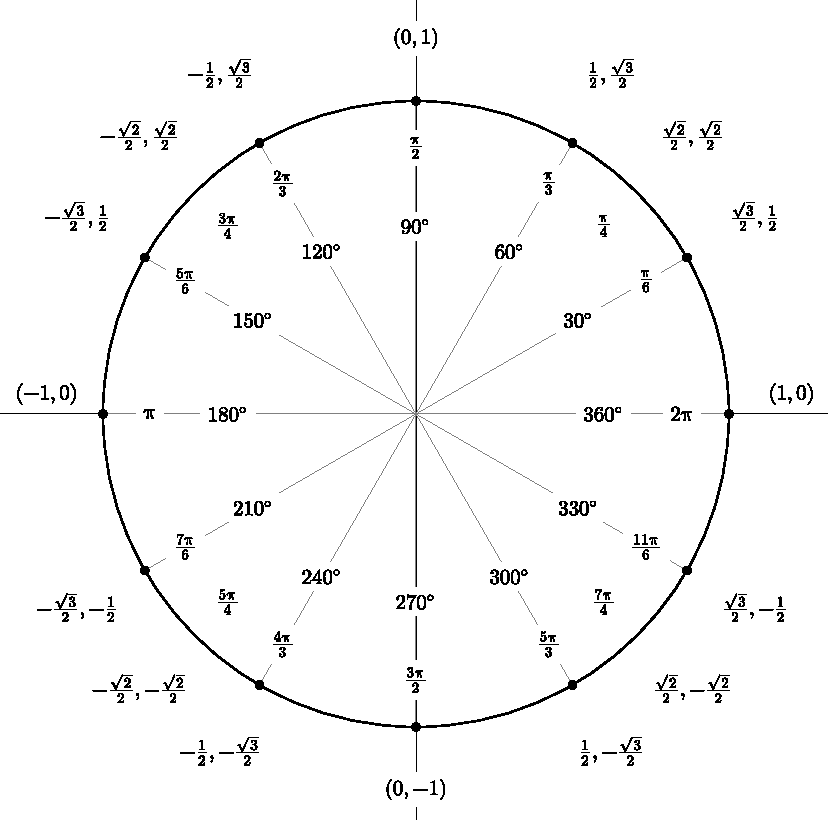
\includegraphics[width=\linewidth]{degrees_circle.pdf}
  
\end{center}

\section{Tabellen}
\subsection{Grenzwerte}
\arraycolsep=1pt\def\arraystretch{1.5}
\begin{center}
  \begin{tabularx}{\linewidth}{XX}
    \toprule
    $\limxi \frac{1}{x} = 0$ & $\limxi 1 + \frac{1}{x} = 1$ \\
    $\limxi e^x = \infty$ & $\limxn e^x = 0$ \\
    $\limxi e^{-x} = 0$ & $\limxn e^{-x} = \infty$ \\
    $\limxi \frac{e^x}{x^m} = \infty$ & $\limxn xe^x = 0$ \\
    $\limxi \ln(x) = \infty$ & $\limxo \ln(x) = -\infty$ \\
    $\limxi (1+x)^{\frac{1}{x}} = 1$ & $\limxo (1+x)^{\frac{1}{x}} = e$ \\
    $\limxi (1+\frac{1}{x})^b = 1$ & $\limxi n^{\frac{1}{n}} = 1$ \\
    $\lim_{x\to\pm\infty} (1 + \frac{1}{x})^x = e$ & $\limxi (1-\frac{1}{x})^x = \frac{1}{e}$ \\
    $\lim_{x\to\pm\infty} (1 + \frac{k}{x})^{mx} = e^{km}$ & $\limxi (\frac{x}{x+k})^x = e^{-k}$ \\
    $\limxo \frac{a^x -1}{x} = \ln(a), \forall a > 0$ &
    $\limxi x^a q^x = 0, \newline \forall 0 \le q < 1$ \\
  \end{tabularx}
  \begin{tabularx}{\linewidth}{XX}
    $\limxo \frac{\sin x}{x} = 1$ & $\limxo \frac{\sin kx}{x} = k$\\
    $\limxo \frac{1}{\cos x} = 1$ & $\limxo \frac{\cos x -1}{x} = 0$ \\
    $\limxo \frac{\log 1 - x}{x} = -1$ & $\limxo x \log x = 0$\\
    $\limxo \frac{1 - \cos x}{x^2} = \frac{1}{2}$ & $\limxo \frac{e^x-1}{x} = 1$ \\
    $\limxo \frac{x}{\arctan x} = 1$ & $\limxi \arctan x = \frac{\pi}{2}$ \\
    $\limxo \frac{e^{ax}-1}{x} = a$ & $\limxo \frac{\ln(x+1)}{x} = 1$ \\
    $\lim_{x\to 1} \frac{\ln(x)}{x-1} = 1$ & $\limxi \frac{\log(x)}{x^a} = 0$ \\
    $\limxi \sqrt[x]{x} = 1$ & $\limxi \frac{2x}{2^x} = 0$ \\
    \bottomrule
  \end{tabularx}
\end{center}
\subsection{Ableitungen}
\begin{center}
  % the c>{\centering\arraybackslash}X is a workaround to have a column fill up all space and still be centered
  \begin{tabularx}{\linewidth}{c>{\centering\arraybackslash}Xc}
  \toprule
  $\mathbf{F(x)}$ & $\mathbf{f(x)}$ & $\mathbf{f'(x)}$ \\
  \midrule
  $\frac{x^{-a+1}}{-a+1}$ & $\frac{1}{x^a}$ & $\frac{a}{x^{a+1}}$ \\
  $\frac{x^{a+1}}{a+1}$ & $x^a \ (a \ne 1)$ & $a \cdot x^{a-1}$ \\
  $\frac{1}{k \ln(a)}a^{kx}$ & $a^{kx}$ & $ka^{kx} \ln(a)$ \\
  $\ln |x|$ & $\frac{1}{x}$ & $-\frac{1}{x^2}$ \\
  $\frac{2}{3}x^{3/2}$ & $\sqrt{x}$ & $\frac{1}{2\sqrt{x}}$\\
  $-\cos(x)$ & $\sin(x)$ & $\cos(x)$ \\
  $\sin(x)$ & $\cos(x)$ & $-\sin(x)$ \\
  $\frac{1}{2}(x-\frac{1}{2}\sin(2x))$ & $\sin^2(x)$ & $2 \sin(x)\cos(x)$ \\
  $\frac{1}{2}(x + \frac{1}{2}\sin(2x))$ & $\cos^2(x)$ & $-2\sin(x)\cos(x)$ \\
  \multirow{2}*{$-\ln|\cos(x)|$} & \multirow{2}*{$\tan(x)$} & $\frac{1}{\cos^2(x)}$  \\
  & & $1 + \tan^2(x)$ \\
  $\cosh(x)$ & $\sinh(x)$ & $\cosh(x)$ \\
  $\log(\cosh(x))$ & $\tanh(x)$ & $\frac{1}{\cosh^2(x)}$ \\
  $\ln | \sin(x)|$ & $\cot(x)$ & $-\frac{1}{\sin^2(x)}$ \\
  $\frac{1}{c} \cdot e^{cx}$ & $e^{cx}$ & $c \cdot e^{cx}$ \\
  $x(\ln |x| - 1)$ & $\ln |x|$ & $\frac{1}{x}$ \\
  $\frac{1}{2}(\ln(x))^2$ & $\frac{\ln(x)}{x}$ & $\frac{1 - \ln(x)}{x^2}$ \\
  $\frac{x}{\ln(a)} (\ln|x| -1)$ & $\log_a |x|$ & $\frac{1}{\ln(a)x}$ \\
  \bottomrule
  \end{tabularx}
\end{center}
\subsection{Weitere Ableitungen}
\begin{center}
  \begin{tabularx}{\linewidth}{>{\centering\arraybackslash}X>{\centering\arraybackslash}X}
  \toprule
  $\mathbf{F(x)}$ & $\mathbf{f(x)}$ \\
  \midrule
  $\arcsin(x)$ & $\frac{1}{\sqrt{1 - x^2}}$ \\
  $\arccos(x)$ & $\frac{-1}{\sqrt{1 - x^2}}$ \\
  $\arctan(x)$ & $\frac{1}{1 + x^2}$ \\ 
  $x^x \ (x > 0)$ & $x^x \cdot (1 + \ln x)$ \\
  \bottomrule
  \end{tabularx}
\end{center}
\subsection{Integrale}
\begin{center}
 \begin{tabularx}{\linewidth}{>{\centering\arraybackslash}X>{\centering\arraybackslash}X}
  \toprule
  $\mathbf{f(x)}$ & $\mathbf{F(x)}$ \\
  \midrule
  $\int f'(x) f(x) \dx$ & $\frac{1}{2}(f(x))^2$ \\
  $\int \frac{f'(x)}{f(x)} \dx$ & $\ln|f(x)|$ \\
  $\int_{-\infty}^\infty e^{-x^2} \dx$ & $\sqrt{\pi}$ \\
  $\int (ax+b)^n \dx$ & $\frac{1}{a(n+1)}(ax+b)^{n+1}$ \\
  $\int x(ax+b)^n \dx$ & $\frac{(ax+b)^{n+2}}{(n+2)a^2} - \frac{b(ax+b)^{n+1}}{(n+1)a^2}$ \\
  $\int (ax^p+b)^n x^{p-1} \dx$ & $\frac{(ax^p+b)^{n+1}}{ap(n+1)}$ \\
  $\int (ax^p + b)^{-1} x^{p-1} \dx$ & $\frac{1}{ap} \ln |ax^p + b|$ \\
  $\int \frac{ax+b}{cx+d} \dx$ & $\frac{ax}{c} - \frac{ad-bc}{c^2} \ln |cx +d|$ \\
  $\int \frac{1}{x^2+a^2} \dx$ & $\frac{1}{a} \arctan \frac{x}{a}$ \\
  $\int \frac{1}{x^2 - a^2} \dx$ & $\frac{1}{2a} \ln\left| \frac{x-a}{x+a} \right|$ \\
  $\int \sqrt{a^2+x^2} \dx $ & $\frac{x}{2}f(x) + \frac{a^2}{2}\ln(x+f(x))$ \\
  \bottomrule
 \end{tabularx}
\end{center}

\begin{mainbox}{Integralformel}
  \vspace{-12pt}
  $$\int_a^b \frac{f(x)}{f(a+b-x)+f(x)}dx = \frac{b-a}{2}$$
  Beweis: 
  $\int_a^b \frac{f(x)}{f(a+b-x)+f(x)}dx = I$
  \\Substitution: $u = a + b -x, du = -dx$
  $$I = \int_b^a \frac{f(a+b-u)}{f(u)+f(a+b-u)}(-du) $$
  $$= \int_a^b \frac{f(a+b-u)}{f(u)+f(a+b-u)}du$$
  $$2 \cdot I = \int_a^b \frac{f(x)+f(a+b-x)}{f(a+b-x)+f(x)}$$
  $$2I = \int_a^b1dx = b-a \implies I = \frac{b-a}{2}$$
\end{mainbox}

\section{Aufgaben}
\subsection{Tipps Für Multiple-Choice}%

\begin{itemize}
	\item \textbf{Richtig lesen!!!}
	\item (Gegen-)Beispiele suchen.
	\hrule
	\item Monotonieverhalten bei verketteten/miteinander verechneten Funktionen bleibt nicht umbedingt erhalten.
    \begin{itemize}
      \item Sei $g: X \to Y$ streng monoton wachsend
      \begin{itemize}
        \item $f: Y \to Z$ (streng) monoton wachsend $\implies$ $f(g(x))$ (streng) monoton wachsend.
        \item $f: Y \to Z$ (streng) monoton fallend $\implies$ $f(g(x))$ (streng) monoton fallend.
      \end{itemize}
      \item Sei $g: X \to Y$ monoton wachsend
      \begin{itemize}
        \item $f: Y \to Z$ (streng) monoton wachsend $\implies$ $f(g(x))$ monoton wachsend.
        \item $f: Y \to Z$ (streng) monoton fallend $\implies$ $f(g(x))$ monoton fallend.
      \end{itemize}
      \item Die Inverse einer monoton wachsenden Funktion ist monoton wachsend.(Beweis mit Umkehrregel)
      \item Die Multiplikation oder Division zweier monotonen Funktionen können monoton wachsend/fallend bleiben oder ihre Monotonie verlieren.
      \item Monoton wachsende Funktion konvex(konkav) $\implies$ Inverse konkav(konvex).
      \item Monoton fallende Funktion konvex(konkav) $\implies$ Inverse konvex(konkav).
    \end{itemize}
	\item Verkettete Funktionen:
		\begin{itemize}
			\item Falls äussere beschränkt $\implies$ Verkettung beschränkt.
			\item Verkettung stetiger Funktionen ist stetig.
			\item Verkettung (streng) konvexer Funktionen, muss nicht konvex sein.
		\end{itemize}
	\item Schauen ob Funktionsfolge $f_n$ \underline{gleichmässig} und nicht nur punktweise gegen $f$ konvergiert.
		$ \implies$ Gewisse Eigenschaften (Stetigkeit) nur dann gültig.
	\item $f''(x_0) = 0 \centernot \implies x_0$ ist ein Sattelpunkt von $f$. 
	\item $f$ stetig $\centernot \implies f'$ stetig.
	\item Sei $f : \R \to \R$ eine ungerade Funktion. $\implies$ $f^{(i)} (0) = 0$ für $i$ gerade.
	\item $X,Y,Z \subset \R$, $f: X \to Y$ und $g: Y \to Z$, sodass $g \circ f : X \to Z$ bijektiv. 
		$\implies$ $f$ injektiv, $g$ surjektiv
	\item Sei $a,b \in \R$ mit $a < b$ mit $f: ]a,b[ \to \R$. Falls $f^2$ und $f^3$ in $]a,b[$
		differenzierbar und $f(x) \neq 0~\forall x \in ]a,b[$ $ \implies$ $f$ in $]a,b[$ differenzierbar. (Da wir $f^3$ durch $f^2$ teilen).
	\item Im Allg. muss eine Grenzfunktion $f$ nicht differenzierbar sein, und wenn sie es ist muss $f'$ nicht gleich $\limn f_n'$ sein.
	
	\item $f: (0,1] \to \R$ monoton $\centernot \implies f$ beschränkt.
	\\ Der Logarithmus $\ln: (0,1] \to \R$ ist monoton, aber nicht beschränkt. 
  \item $f: [a, b] \to \R$ für beliebige $a, b \in \R, a < b$ ist beschränkt.
  \item $f(x) = |x| \cdot \text{sign}(x)$ ist stetig, da $|x| \cdot \text{sign}(x) = x$ und $g(x)=x$ stetig.
\end{itemize}

\subsection{Multiple Choice}

Sei $a, b \in \R$ mit $a < b$ und $f : [a, b] \to \R$ eine Funktion. Sei $f_n : [a, b] \to R, n \geq 1$ so
dass die Funktionenfolge $(f_n)n \geq 1$ auf $[a, b]$ gleichmässig gegen $f$ konvergiert. Geben Sie
für jede folgender Aussagen an ob sie wahr oder falsch ist.
\begin{enumerate}
\item Sei $x_0 \in ]a, b[$ . Falls $f_n$ für alle $n \geq 1$ in $x_0$ differenzierbar ist, so ist $f$ in
$x_0$ differenzierbar.
\\(A) wahr.
\\\textbf{(B) falsch.}
\\ Stetigkeit $\centernot \implies$ Differenzierbarkeit
\item Falls $f_n$ für alle $n \geq 1$ auf $[a, b]$ beschränkt ist dann folgt, dass für jede
Partition $P$ von $[a, b]$ der Grenzwert der Untersumme $\limn s(f_n, P)$
 existiert und $\limn s(fn, P) = s(f, P)$.
\\\textbf{(A) wahr.}
\\(B) falsch.
Sei $P=\{x_0, ..., x_m\}$ eine Partition von $[a,b]$ mit $x_0 < ... < x_m$
$\\ \lim \limits_{n\to\infty}s(f_n,P)=\lim \limits_{n\to\infty} \sum\limits_{i=1}^{m}\inf\limits_{x_{i-1}\leq x\leq x_i}f_n(x) \delta_{i} =\sum\limits_{i=1}^{m}\inf\limits_{x_{i-1}\leq x\leq x_i}\lim \limits_{n\to\infty}\left(f_n(x)\right)\delta_{i}
\\=\sum\limits_{i=1}^{m}\inf\limits_{x_{i-1}\leq x\leq x_i}f(x)\delta_{i} =\sum\limits_{i=1}^{m}f_i \delta_i=s(f,P)$
\item Falls fn für alle $n \geq 1$ stetig ist, so ist $f$ gleichmässig stetig.
\\\textbf{(A) wahr.}
\\(B) falsch.
\\ gleichmässige Konvergenz $\implies$ Stetigkeit von $f$ $\implies$ gleichmässige Stetigkeit da kompaktes Intervall 
\item Falls $f_n$ für alle $n \geq 1$ konvex ist, so ist $f$ konvex.
\\\textbf{(A) wahr.}
\\(B) falsch.
\end{enumerate}

\vspace{0.1 cm}
\hrule
\vspace{0.2 cm}

Sei $(q_n)_{n \geq 1}$ eine Folge rationaler Zahlen, sodass
\\$|q_n - q_n+1| \to 0$ für $n \to \infty$.
\\Dann ist $(q_n)_{n \in \N}$ eine Cauchy-Folge.
 \\ 
\\\textbf{Falsch:} Sei $q_n = \sum_{k = 1}^n \frac{1}{k}$. Dann ist $q_n \in \mathbb{Q}$ und es gilt $|q_n - q_{n+1}| = |- \frac{1}{n+1}| \to 0$ für $n \to \infty$, 
aber $(q_n)_{n \in \N}$ ist keine Cauchy-Folge, denn $$q_{2n} - q_n = \frac{1}{n+1} + \dots + \frac{1}{2n} \geq \frac{n}{2n} = \frac{1}{2}$$

\vspace{0.1 cm}
\hrule
\vspace{0.2 cm}

Sei $(a_n)_{n \geq 1}$ eine konvergente Folge, und $\sigma$ eine Permutation von $\left\{1, 2, 3, \dots \right\}$
(d.h. eine Bijektion der Menge $\left\{1, 2, 3, \dots \right\}$ auf sich selbst). Dann konvergiert auch die Folge $b_n = a_{\sigma(n)}, \forall n \geq 1$.
\\ 
\textbf{Richtig.} Sei $\alpha \in \R$ der Grenzwert der Folge$(a_n)_{n \geq 1}$. Es gilt $\forall \varepsilon < 0, \exists N_\varepsilon: |\alpha - a_n| < \varepsilon, \forall n \geq N_\varepsilon$.
\\ Wir definieren $m_\varepsilon = \max ({k: \sigma(k) \leq n_\varepsilon})$. Es gilt $m_\varepsilon < \infty$, da $n_\varepsilon < \infty$ und $\sigma$ eine Bijektion. Dann gilt:
$$|\alpha - b_n| = |\alpha - a_{\sigma(n)}| < \varepsilon, \forall n \geq m_\varepsilon$$
Somit folgt $\limn b_n = \alpha$.

\vspace{0.1 cm}
\hrule
\vspace{0.2 cm}

  Sei $\phi: \N^* \to \N^*$ eine Abbildung, $\sumn a_n$ eine Reihe und $b_n = a_{\phi(n)}$.
  \begin{enumerate}
    \item $\sumn a_n$ ist konvergent und $\phi$ surjektiv $\implies \sumn b_n$ ist konvergent.
    \\\textbf{Falsch}. Gegenbeispiel:
     $$\sumn a_n = 1 + \left(-1\right) + \frac{1}{2} + \left(-\frac{1}{2}\right) + \frac{1}{3} + \dots$$
     konvergiert, aber
     $$\sumn b_n = 1 + 1 + \left(-1\right) + \frac{1}{2} + \frac{1}{2} + \left(-\frac{1}{2}\right) + ...$$
     konvergiert nicht.
    \item $\sumn a_n$ ist konvergent und $\phi$ injektiv $\implies \sumn b_n$ ist konvergent.
    \\\textbf{Falsch}. Gegenbeispiel:
     $$\sumn a_n = 1 + \left(-1\right) + \frac{1}{2} + \left(-\frac{1}{2}\right) + \frac{1}{3} + \dots$$
     konvergiert, aber
     $$\sumn b_n = 1 + \frac{1}{2} + \frac{1}{3} + ...$$
     konvergiert nicht.
     \item $\sumn a_n$ ist absolut konvergent und $\phi$ surjektiv $\implies \sumn b_n$ ist konvergent.
     \\\textbf{Falsch}. Gegenbeispiel:
      $$\sumn a_n = 1 + \frac{1}{2} ) + \frac{1}{4} + \frac{1}{8} + \dots$$
      konvergiert, aber
      $$\sumn b_n = 1 + 1 + \frac{1}{2} + \frac{1}{2} + \frac{1}{4} + ...$$
      konvergiert nicht.
      \item $\sumn a_n$ ist absolut konvergent und $\phi$ injektiv $\implies \sumn b_n$ ist konvergent.
     \\\textbf{Richtig}. Eine Teilfolge oder eine Umordnung der absolut konvergenten Reihe ist auch absolut konvergent.
  \end{enumerate}

\vspace{0.1 cm}
\hrule
\vspace{0.2 cm}

Sei $\sumk a_k$ absolut konvergent und $\sumk b_k$ konvergent.
\begin{itemize}
  \item Die Reihe $\sumk |a_k|^2$ konvergiert immer absolut.
  \item Die Reihe $\sumk a_kb_k$ konvergiert immer absolut.
  \item Beweis: $(a_k)$ und $(b_k)$ sind beschränkt. Dann $\exists C > 0, |a_k| + |b_k| < C$ und 
  \\$|a_k|^2 < C|a_k|, |a_kb_k| < C|a_k|$.
\end{itemize}

\vspace{0.1 cm}
\hrule
\vspace{0.2 cm}

Sei $I$ ein Intervall und $f: I \to \R$ eine stetige Funktion:
\begin{itemize}
  \item $I$ kompakt $\implies$ $f(I)$ kompakt.
  \item $f(I)$ kompakt $\centernot \implies I$ kompakt.
  \\ Gegenbeispiel: Sei $I = (-\pi, \pi)$ und $f(x)= \sin x$. Dann ist $f(I) = [-1, 1]$ kompakt, aber $(-\pi,\pi)$ ist nicht kompakt.  
\end{itemize}

\vspace{0.1 cm}
\hrule
\vspace{0.2 cm}

Wir betrachten die Funktionenfolge $(f_n)$ mit 
$$f_n: \R_{\geq 0} \to \R, x \to (x^{\frac{1}{2}}+n^{-1})^2$$
\begin{itemize}
  \item $\limn f_n(x) = x$ für alle $x \in \R_{\geq 0}$
  \item Die Funktionenfolge konvergiert gleichmässig.
  \\ \textbf{Falsch}: Aus $|f_n(x) - x| = 2\frac{x^{\frac{1}{2}}}{n} + \frac{1}{n^2}$ folgt, dass für $x > n^2, |f_n(x) - x| > 2$. Folglich kann $(f_n)$ nicht gleichmässig konvergieren.
  \item Für alle $M > 0$ gilt, dass $f_n|_{[0, M]}: [0,M] \to \R$ gleichmässig konvergiert.
  \\ \textbf{Richtig}: Es gilt $|f_n(x) - x| = 2\frac{x^{\frac{1}{2}}}{n} + \frac{1}{n^2} \leq M^{\frac{1}{2}} + \frac{1}{n^2}, \forall x \in [0,M]$.\\Da $\limn \left(\frac{2M^{\frac{1}{2}}}{n} + \frac{1}{n^2}\right) = 0$, konvergiert $(f_n|_{[0.M]})$ gleichmässig.  
\end{itemize}

\vspace{0.1 cm}
\hrule
\vspace{0.2 cm}

Falls $f_n$ eine Funktionenfolge ist, wobei $f_n$ für jedes $n \in \N$ einmal stetig differenzierbar ist und falls sowohl $(f_n)$ als auch $(f_n')$ gleichmässig konvergieren, mit $f_n \to f$ und $f_n' \to g$, dann ist $f$ stetig differenzierbar mit $f' = g$.

\vspace{0.1 cm}
\hrule
\vspace{0.2 cm}

Sei $f: \R \to \R$ eine beliebig oft stetig differenzierbare Funktion. Welche der folgenden Aussagen ist im Allgemeinen nicht richtig?
\begin{enumerate}
  \item $f$ hat eine Taylorreihe bei $x_o = 0$
  \item Der Konvergenzradius der Taylorreihe ist $\geq 0$, aber nicht notwendig $>0$
  \item Dort, wo die Taylorreihe konvergiert, stellt sie die Funktion $f$ dar.
  \item Wenn $f$ durch eine Potenzreihe gegeben ist, so ist diese gleich der Taylorreihe.
\end{enumerate}
\textbf{Lösung:} (3) ist falsch. Gegenbeispiel: 
\\Sei $f$ eine Funktion mit $f(0) = 0$ und $f(x)=e^{-1/x^2}$ für $x \neq 0$. 
\\Diese ist beliebig oft stetig differenzierbar, aber ihre Taylorreihe mit Entwicklungspunkt $x_0 = 0$ ist immer gleich $0$ und weicht daher von der Funktion $f$ für $x \neq 0$ ab.

\vspace{0.1 cm}
\hrule
\vspace{0.2 cm}

Seien $f, g: [0, \infty[ \to \R$ nicht negative, zweimal differenzierbare Funktionen. Die Funktion $h$ sei definiert durch $h(x) := g(f(x))$ für alle $x \geq 0$.
\begin{enumerate}
  \item $h$ ist zweimal differenzierbar.
  \\ \textbf{Wahr}: $h''(x) =  g''(f(x)) \cdot f'(x)^2 + g'(fx(x))\cdot f''(x)$
  \item Wenn $f$ und $g$ streng konvex sind, ist $h$ konvex.
  \\ \textbf{Falsch:} Gegenbeispiel mit $f(x) = g(x) = (x-1)^2$
  \item Wenn $\int_0^\infty f(x)\dx$ und $\int_0^\infty g(x)\dx$ konvergieren, konvergiert $\int_0^\infty h(x)\dx$.
  \\ \textbf{Falsch:} Gegenbeispiel $f(x) = g(x) = e^{-x}$. Dann gilt $\int_0^\infty f(x)\dx=\int_0^\infty g(x)\dx = 1$.
  \\Da aber $$\limxi h(x) = \limxi e^{(-e^{-x})} = \limxi \frac{1}{e^{\frac{1}{e^x}}} = 1$$ divergiert $\int_0^\infty h(x) \dx$.
\end{enumerate}

\subsection{Versch. Aufgaben}%


	Zeigen sie, dass für alle $t \in \R$ gilt:
	\begin{equation*}
		\lim_{n \to \infty} \left( \cos \left( \frac{t}{\sqrt{n}} \right) \right)^n = e^{-\frac{t^2}{2}}
	\end{equation*}
	
	Reihenentwicklung: $\cos (x) = 1 - \frac{x^2}{2} + \oof \left(x^4 \right)$ und\\$\ln (1+x) = x + \oof \left(x^2 \right)$.
	\begin{align*}
	\cos \left( \frac{t}{\sqrt{n}} \right)^n &= \exp \left( n \log \left( \cos \left( \frac{t}{\sqrt{n}}  \right) \right) \right)\\ 
						 &= \exp \left( n \log \left( 1 - \frac{t^2}{2n} + \oof \left( \frac{1}{n^2} \right) \right) \right)\\
						 &= \exp \left( n \left( - \frac{t^2}{2n} + \oof \left( \frac{1}{n^2} \right) \right) \right)\\
						 &= \exp \left( - \frac{t^2}{2} + \oof \left( \frac{1}{n} \right) \right)\\
						 & \underset{n \to \infty}{\longrightarrow} \exp \left( - \frac{t^2}{2} \right) = e^{-\frac{t^2}{2}}
	\end{align*}

\vspace{0.1 cm}
\hrule
\vspace{0.2 cm}


  Berechne $\int_{-\infty}^{+\infty} \sin(x)\exp\left(-x^2\right) dx$
	
	Wir wissen $\sin(x)$ ungerade und $\exp\left(-x^2\right)$ gerade.
	\\Das Produkt einer ungeraden und geraden Funktion ist eine ungerade Funktion.\\
	Für ungerade Funktionen gilt $$\int_{-a}^{+a} f(x) \dx = 0$$ Daraus folgt: 
	$\int_{-\infty}^{+\infty} \sin(x)\exp\left(-x^2\right) \dx = 0$

\vspace{0.1 cm}
\hrule
\vspace{0.2 cm}


  Sei $x$ und $\theta$ reelle Zahlen mit $x + \frac{1}{x} = 2 \cos(\theta)$.
	Zu zeigen: Für jede natürliche Zahl $n \geq 1$ gilt
	\begin{equation*}
		x^n + \frac{1}{x^n} = 2 \cos (n \theta)
	\end{equation*}
	
	\textbf{IA}%
	\begin{align*}
		n=2:~x^2 + \frac{1}{x^2} = \left( x + \frac{1}{x} \right)^2 -2 \\= 4 \cos^2 (\theta) -2
					 = 2 \left( 2 \cos^2 (\theta) -1 \right) \\
           = 2 \left( \cos^2 (\theta) - \left( 1 - \cos^2 (\theta) \right) \right)\\
					 = 2 \left( \cos^2 (\theta) - \sin^2 (\theta) \right) = 2 \cos (2 \theta)
	\end{align*}
	\textbf{IH}%
	\\gilt für $n=k$ und $n=k+1$\\
   \\
	\textbf{IS}%
	
		$$x^{k+2} + \frac{1}{x^{k+2}} = \left( x^{k+1} + \frac{1}{x^{k+1}} \right)\left( x + \frac{1}{x} \right)$$ 
    \\$$- \left( x^{k} + \frac{1}{x^{k}} \right) = 4 \cos \left( (n+1) \theta \right) \cos(\theta)$$ 
     \\$$- 2 \cos (n \theta) \overset{\text{\textcolor{blue}{$(*)$}}}= 4 \cos \left( (n+1) \theta \right) \cos(\theta)$$ 
     \\$$- 2 \left( \cos \left( (n+1) \theta \right) \cos(-\theta) 
    - \sin \left( (n+1) \theta \right) \sin(-\theta) \right)$$\\
		$$= 2 \cos \left( (n+1) \theta \right) \cos(\theta) - 2 \sin \left( (n+1) \theta \right) \sin (\theta)$$
    \\$$\overset{\text{Add.T.}}{=} 2 \cos \left( (n+2) \theta \right)$$
	
	Der Schritt \textcolor{blue}{$(*)$} lässt sich folgendermassen berechnen:
	\begin{align*}
		\cos(n \theta) 
    &= \cos (n\theta + \theta -\theta)\\ 
    &= \cos(n \theta + \theta) \cos(-\theta) - \sin(n \theta + \theta ) \sin ( -\theta)
	\end{align*}

\vspace{0.1 cm}
\hrule
\vspace{0.2 cm}

Manipulation für $f(x) = \sin(\arctan (x))$ (funktioniert ähnlich für $\cos(\arctan (x))$):

\begin{align*}
  f(x) &=\frac{\sin(\arctan(x))}{\sqrt{\sin^2(\arctan(x))+\cos^2(\arctan(x))}}\\
  &=\frac{\frac{\sin(\arctan(x))}{\cos(\arctan(x))}}{\sqrt{\frac{\sin^2(\arctan(x))}{\cos^2(\arctan(x))}+1}}\\
  &=\frac{\tan(\arctan(x))}{\sqrt{\tan^2(\arctan(x))+1}}\\
  &=\frac{x}{\sqrt{x^2+1}}
\end{align*}

Manipulation für $f(x) = \tan(\arcsin (x))$:
\begin{align*}
  f(x)&=\tan(\arcsin (x))\\
  &=\frac{\sin(\arcsin(x))}{\cos(\arcsin(x))}\\
  &=\frac{\sin(\arcsin(x))}{\sqrt{1-\sin^2(\arcsin(x))}}\\
  &=\frac{x}{\sqrt{1-x^2}}.
  \end{align*}

\vspace{0.1 cm}
\hrule
\vspace{0.2 cm}
\begin{align*}
  \int x\arcsin(x)\,\mathrm dx\\
\end{align*}
Substitution mit $ x = \sin(u) $:
\begin{align*}
  =\int \sin(u)\cos(u) u \, \mathrm du\\
  = \int \frac{1}{2} sin(2u) u \, \mathrm du\\
  = \frac{1}{2} \int \sin(2u) u \, \mathrm du\\
\end{align*}
 Partielle Integration ( $u$ ableiten, $\sin(2u)$ integrieren):
 \begin{align*}
  \frac{1}{2} \int u \sin(2u)\, \mathrm du \\ 
  = \frac{1}{2} \left[ u \cos(2u)  \left(-\frac{1}{2}\right) - \int \left(-\frac{1}{2}\right) \cos(2u) \, \mathrm du \right] \\ 
  =-\frac{1}{4} u \cos(2u) + \frac{1}{4} \int \cos(2u) \, \mathrm du\\
  = -\frac{1}{4} u \cos(2u) + \frac{1}{8} \sin(2u) + C
\end{align*}
$u = \arcsin(x)$ einsetzen liefert:
$$= -\frac{1}{4} \arcsin(x) \cos(2\arcsin(x)) + \frac{1}{8} \sin(2\arcsin(x)) + C$$

\vspace{0.1 cm}
\hrule
\vspace{0.2 cm}

Let us take $k_0\in\mathbb N$ large enough so that $\sqrt{\lvert t\rvert}<k_0$. Then there is $1+t/k^2>0$ for all $k\geq k_0$. It is now sufficient to show that
$$
\lim_{n\to\infty}\prod_{k=k_0}^n\left(1+\frac t{k^2}\right)
$$
exists because if it does, the original limit is this limit times
$$
\prod_{k=1}^{k_0-1}\left(1+\frac t{k^2}\right),
$$
which is a finite product (and thus a finite constant).

Since $e^x$ and $\ln(x)$ are continuous, showing that
$$
\lim_{n\to\infty}\prod_{k=k_0}^n\left(1+\frac t{k^2}\right)
$$
exists is equivalent to showing that
$$
\lim_{n\to\infty}\ln\left(\prod_{k=k_0}^n\left(1+\frac t{k^2}\right)\right)
$$
exists. Note that the $\ln$ here is well defined because the product is a product of positive numbers and thus positive itself. We have
$$
\ln\left(\prod_{k=k_0}^n\left(1+\frac t{k^2}\right)\right)=\sum_{k=k_0}^n\ln\left(1+\frac t{k^2}\right),
$$
so we just need to show that
$$
\lim_{n\to\infty}\sum_{k=k_0}^n\ln\left(1+\frac t{k^2}\right)
$$
exists -- in other words, that
$$
\sum_{k=k_0}^\infty\ln\left(1+\frac t{k^2}\right)
$$
converges.

We can approximate $\ln\left(1+\frac t{k^2}\right)\approx\frac t{k^2}$. More precisely,
\begin{align*}
\lim_{k\to\infty}\frac{\frac t{k^2}}{\ln\left(1+\frac t{k^2}\right)}=\lim_{\ell\to0^+}\frac{t\ell}{\ln\left(1+t\ell\right)}=\lim_{\ell\to0^+}\frac{t}{\frac t{1+t\ell}}\\=\frac tt=1.
\end{align*}
Therefore, $\sum_{k=k_0}^\infty\ln\left(1+\frac t{k^2}\right)$ converges if and only if $\sum_{k=k_0}^\infty\frac t{k^2}$ converges. However, we actually know that
$$
\sum_{k=k_0}^\infty\frac t{k^2}=t\left(\zeta(2)-\sum_{k=1}^{k_0-1}\frac1{k^2}\right)=t\left(\frac{\pi^2}6-\sum_{k=1}^{k_0-1}\frac1{k^2}\right)
$$
does converge.

\vspace{0.1 cm}
\hrule
\vspace{0.2 cm}

Berechnen Sie die Integral $\int_1^2 \frac{1}{x^2}\dx$ per Definition.
\textbf{Lösung}: Sei $f(x) = \frac{1}{x^2}$, 
\\$P_n = \left\{x_k := 1 + \frac{k}{n} \mid k \in \left\{0, 1, \dots, n-1\right\} \right\}$,
\\$\xi = \left\{\xi_k := \sqrt{x_k \cdot x_{k+1}} \mid k \in \left\{0, 1, \dots, n-1\right\}\right\}$
\\Dann gilt
\begin{align*}
  S(f, P_n, \xi) &= \sum_{k = 0}^{n - 1} f(\xi_k)\cdot(x_{k+1}-x_k)\\
                 &= \sum_{k = 0}^{n - 1} \frac{1}{x_k \cdot x_{k+1}} \cdot \frac{1}{n}\\
                 &= \sum_{k = 0}^{n - 1} \frac{n^2}{(k + n)(k + n + 1)}\cdot \frac{1}{n}\\
                 &= n \cdot \sum_{k = 0}^{n - 1} \frac{1}{(k + n)(k + n + 1)}\\
                 &= n \cdot \sum_{k = 0}^{n - 1} \left(\frac{1}{k + n} - \frac{1}{k + n + 1}\right)\\
                 &= n \cdot \left(\frac{1}{n}-\frac{1}{2n}\right) = \frac{1}{2}\\
\end{align*}
$$\int_1^2 \frac{1}{x^2}\dx = \limn S(f, P_n, \xi) = \limn \frac{1}{2} = \frac{1}{2}$$

\vspace{0.1 cm}
\hrule
\vspace{0.2 cm}

Zeige $\int_1^{n+1} \frac{\sin(\pi x)}{\lfloor x\rfloor}\dx = -\frac{2}{\pi}\sum_{k=1}^{n}\frac{(-1)^{k-1}}{k}$

Sei $$\int_1^{n+1} \frac{\sin(\pi x)}{\lfloor x\rfloor}\dx = \sum_{k=1}^{n} I_k$$ 
mit $$I_k = \int_k^{k+1}\frac{\sin(\pi x)}{\lfloor x\rfloor}\dx$$
\begin{align*}
  I_k &= \int_k^{k+1} \frac{\sin(\pi x)}{k}\dx = \frac{1}{k}\cdot\frac{1}{\pi}\cdot \left(-\cos(\pi x)\right)\mid_k^{k+1}\\
      &= \frac{\cos(k\pi) - \cos((k+1)\pi)}{k\pi} = \frac{2(-1)^k}{k\pi}\\ 
\end{align*}
Daraus folgt
$$\int_1^{n+1} \frac{\sin(\pi x)}{\lfloor x\rfloor}\dx = \sum_{k=1}^{n}\frac{2(-1)^k}{k\pi} = -\frac{2}{\pi}\sum_{k=1}^{n}\frac{(-1)^{k-1}}{k}$$

\vspace{0.1 cm}
\hrule
\vspace{0.2 cm}

Beweise die Konvergenz von $\int_{0}^1 \frac{\sin \frac{1}{x}}{x^{3/2}} \dx$
\\Mit partieller Integration:
\begin{align*}
  \int_a^1 \frac{\sin \frac{1}{x}}{x^{3/2}}\dx &= \int_a^1 \frac{\sin\frac{1}{x}}{x^2}\cdot \sqrt{x} \dx\\
                                               &= \cos\left(\frac{1}{x}\right)\cdot\sqrt{x}\bigg|_a^1 - \int_a^1 \cos\left(\frac{1}{x}\right) \cdot \frac{1}{2\sqrt{x}}\dx\\
                                               &= \cos(1) - \sqrt{a}\cos\left(\frac{1}{a}\right) - \frac{1}{2} \int_a^1 \frac{\cos\left(\frac{1}{x}\right)}{\sqrt{x}}\dx                                              
\end{align*}
Es gilt $\lim_{a \to 0} \cos1 - \sqrt{a}\cos\frac{1}{a} = \cos 1$.
Also müssen wir nur noch die Konvergenz von $\int_a^1\frac{\cos \frac{1}{x}}{\sqrt{x}}\dx$ zeigen.
Da $\frac{-1}{\sqrt{x}} \leq \frac{\cos \frac{1}{x}}{\sqrt{x}} \leq \frac{1}{\sqrt{x}}$ und $\int_0^1 \frac{1}{\sqrt{x}}\dx$ konvergiert, konvergiert dieses Integral.

\vspace{0.1 cm}
\hrule
\vspace{0.2 cm}

Untersuche die Konvergenz von $\int_1^{+\infty} \sin\left(\frac{1}{x}\right)\dx$.
\\Substitution: $t = \frac{1}{u}, \dx = \frac{1}{u^2} \text{d}u$
\\Mittels Taylorentwicklung gilt: $\sin u = u - \frac{u^3}{6}\cos \tau$ für ein $\tau \in [0, u]$
\begin{align*}
  \int_0^1 \frac{\sin u}{u^2}\text{d}u &= \int_0^1 \frac{1}{u} - \frac{\cos \tau}{6}u\text{d}u = \ln u -\frac{\cos(\tau) u^2}{12} \bigg|_0^1\\
                                       &= \ln 1 - \frac{\cos(\tau)1^2}{12} - \lim_{a \to 0}\left(\ln a - \frac{\cos(\tau)a^2}{12}\right)\\
                                       &= 0 - \frac{\cos(\tau)}{12} - \lim_{a \to 0}\left(\ln a\right) + 0\\
                                       &= -\infty
\end{align*}
Demzufolge ist $\int_1^{+\infty} \sin\left(\frac{1}{x}\right)\dx$ divergent.

\vspace{0.1 cm}
\hrule
\vspace{0.2 cm}

Bestimmen Sie mit Hilfe des linearen Taylorpolynoms um $t_0 = 8$ eine Näherung
an $\sqrt[3]{7}$.
\\Geben Sie eine Abschätzung für den Fehler dieser Näherung an.
\\Für $f(t) = \sqrt[3]{t}$ ist $f'(t) = \frac{1}{3}t^{-\frac{2}{3}}$.
\\$\implies$ 
$$T_1(f, t, 8) = f(8) + f'(8)(t - 8) = 2 + \frac{1}{3}\left(\frac{1}{2}\right)^2 \cdot (t- 8)$$ 
Näherung für $\sqrt[3]{7} = T_1(f, 7, 8) = 2 - \frac{1}{12} = \frac{23}{12}$
\\Fehlerabschätzung:
$$R_1(f, t, t_0) = \frac{f''(\xi)}{2!}(t - t_0)^2 = \frac{f''(\xi)}{2!}(7-8)^2 = \frac{f''(\xi)}{2}$$
für ein $\xi \in [7, 8]$.
Da $f''(t) =-\frac{2}{9} t^{-\frac{5}{3}}$ gilt:
$$|\text{Fehler}| \leq \frac{1}{2} \sup_{\xi \in [7, 8]} |f''(\xi)| = \frac{1}{2}\cdot \frac{2}{9} \cdot \frac{1}{7^{5/3}} = \frac{1}{9 \cdot 7^{5/3}}.$$

\section{Quellen}
Diese Cheatsheet wurde stark von verschiedenen schon vorhandenen Zusammenfassungen inspiriert (Julian Steinmann, Danny Camenisch, Andrej Scheuer etc.). 
\\ \\
Auch sind die meisten Aufgaben und deren Lösungen von den VIS Community Solutions übernommen worden.
\\ \\
Die Definitionen sind meistens dem Skript“Analysis 1” von Marc Burger und den Vorlesungsnotizen von Analyis 1 im Frühlingssemester 2022 entnommen.
\\ \\
Ich wünsche allen viel Erfolg!

\end{document}
